\chapter[Background material]{Background material: from gradient to identification.}
\label{ch:basics}
\etocsettocstyle{\subsubsection*{Chapter Contents}}{}
\localtableofcontents
\newpage
\section*{Introduction}
\addcontentsline{toc}{section}{Introduction}
Mathematical optimization is a tool to chose some ``optimal'' parameter $x$ within the \emph{constraint set} $X$ such that it minimizes \emph{objective} function $f$. More formally, an optimization problem could be written in the following general form
$$
\min_{x\in X} f(x),
$$
that corresponds to a lot of practical applications in \dg{areas} such as: bioinformatics, advertising, visual object recognition, and other applications. However, this problem is general and there is no general algorithm to solve this problem.

To produce an efficient algorithm with guarantee\dg{s} to solve the problem some additional assumptions of $f$ and $X$ are commonly added. One of the common assumptions is \dg{the} convexity of objective function and constraint set. In our work, we consider convex functions $f:\RR^n\rightarrow \RR\cup\{+\infty\}$ and $X = \RR^n$, and in this chapter, we present an important background to discover new algorithms.

In order to make good prediction\dg{s} large-scale data is used when training the models: the number of observations $m$ is large and the dimension of each observation (or the number of features) $n$ is big. It raises a lot of questions, including, how to make the existing optimization algorithms computationally more efficient? In this context, classical optimization methods like gradient descent and its variations \dg{are} computationally expensive, because every step of these algorithms requires \dg{a} pass through the full dataset. In contrast, incremental methods, that use a single data point \dg{(or a minibatch)} to compute an estimator for the gradient reduce the computational cost of iteration. However,  state-of-the-art algorithms are distributed to accept bigger datasets. In such algorithms, the communication process between machines is also expensive process and methods that \dg{can} reduce the amount of communications or the size of every single update are \dg{sought after}.

\mitya{
\paragraph{Outline.} This chapter is organized as follows. In Section \ref{sec:basics_convex}, we introduce basic definitions from convex optimization. Furthermore, we recall some first-order optimization methods and theoretical results that we use in later chapters. \dg{In Section \ref{sec:basics_intro}, we discuss Machine Learning.} In Section \ref{sec:distributed-intro}, we present an overview of distributed learning : setting, context, methods. In particular, we recall the asynchronous distributed proximal algorithm \cite{ICML18}. We present in Section \ref{sec:basics_identificationn}, an active-set identification property and prove this result for this algorithm.  
}
\section{Convex optimization}\label{sec:basics_convex}
\mitya{
In this section, we \dg{provide a} convex optimization background.%, that next chapters assume to be known.
In Subsection \ref{sec:basics_conv_and_smoothness}, we introduce the definitions of convex, strongly-convex, and $L$-smooth (with $L$-Lipschitz gradient) functions and prove some important properties, that are widely used in our further theoretical proofs. In Subsection \ref{sec:basics_gd}, we recall the \emph{Gradient Descent} algorithm (see Algorithm \ref{algo:gd}) and \dg{its} convergence. In Subsection \ref{sec:basics_nonsmooth}, we present the notion of \emph{subgradient}, \emph{proximal operator}, and \emph{Moreau-Yosida regularization}. Furthermore, we recall the basic methods for the minimization of non-smooth functions: \emph{Subgradient Descent} (see Algorithm \ref{algo:sd}) and \emph{Proximal Minimization} (see Algorithm \ref{algo:pm}). Finally, in Subsection \ref{sec:basics_nonsmooth}, we overview the optimization methods to solve regularized \dg{Empirical Risk Minimization problem}: \emph{Coordinate Descent} (see Algorithm \ref{algo:cd_composite}), \emph{Proximal Gradient Descent} (see Algorithm \ref{algo:pgd}), and \emph{Stochastic Gradient Descent} variations.
}
\subsection{Convexity and smoothness}\label{sec:basics_conv_and_smoothness}
In this section, we recall the basic definitions and properties that are used to analyse optimization methods for smooth and convex objective \cite{hiriart2012fundamentals}. 
\begin{definition}[Convex function]
A function $f:\RR^n\rightarrow \RR\cup{+\infty}$ is called convex if $\dom f$ is a convex set and for any $x, y\in \dom f$ and $\alpha \in[0,1]$
\begin{equation}\label{eq:conv_def}
f(\alpha x + (1-\alpha)y)\leq \alpha f(x) + (1-\alpha)f(y),
\end{equation}
where the domain of function $f$ is defined as
$$
\dom f = \{x:|f(x)|<\infty\}.
$$
Moreover, function $f$ is called $\mu$-strongly convex if function $g = f - \frac{\mu}{2}\|x\|_2^2$ is convex.
\end{definition}

From this definition, we could immediately get the following interpretation for smooth functions $f$ that is more practical for further analysis. 

\begin{lemma}\label{lm:convex}[Theorem $2.1.2$ \cite{nesterov-book}]
    A continuously differentiable function $f:\RR^n\rightarrow \RR\cup{+\infty}$ is convex iff for any $x,y\in\mathbb{R}^n$, we have
    \begin{equation}\label{eq:convex_1}
        f(y) \geq f(x) + \langle \nabla f(x), y-x\rangle.
    \end{equation}
    Moreover, function $f:\RR^n\rightarrow \RR\cup{+\infty}$ is $\mu$-strongly convex iff for any $x,y$ in $\mathbb{R}^n$, we have
    \begin{equation}\label{eq:convex_2}
        f(y) \geq f(x) + \langle \nabla f(x), y-x\rangle + \frac{\mu}{2}\|y-x\|_2^2.
    \end{equation}
\end{lemma}
\begin{proof}[Proof of Lemma \ref{lm:convex}]
If $f$ is a convex function then for any $\alpha\in[0,1]$ we have 
$$
f(y)\geq f(x) +\frac{1}{1-\alpha}\left(f(\alpha x + (1-\alpha)y) - f(x)\right),
$$
where the computation of limit for $\alpha \rightarrow 1$ will give \eqref{eq:convex_1}.

Let us now prove the convexity of $f$ form \eqref{eq:convex_1}.
Summing the following inequalities with multipliers $\alpha$ and $1-\alpha$ correspondingly
$$
f(\alpha x + (1-\alpha)y) \leq f(x) - \langle \nabla f(\alpha x + (1-\alpha)y), (1-\alpha)(x-y)\rangle = f(x) + (1-\alpha) \langle \nabla f(\alpha x + (1-\alpha)y), y-x\rangle
$$
$$
f(\alpha x + (1-\alpha)y) \leq f(y) - \langle \nabla f(\alpha x + (1-\alpha)y), \alpha(y-x)\rangle = f(x) - \alpha \langle \nabla f(\alpha x + (1-\alpha)y), y-x\rangle
$$
we immediately get \eqref{eq:conv_def}. 

The proof of \eqref{eq:convex_2} immediately follows from the definition of the strong convexity.
\end{proof}

Convexity implies that any stationary point is a global minima of $f$. In addition, the strong convexity implies the existence and uniqueness of $x^\star = \argmin_{x\in\mathbb{R}^n} f(x)$.

Now let us recall the definition of the $L$-smoothness. 

\begin{definition}[$L$-smoothness]
Differentiable function $f$ is called $L$-smooth if its gradient is $L$-Lipschitz
\begin{equation}
    \|\nabla f(x) - \nabla f(y)\|_2\leq L\|x-y\|_2
\end{equation}
for any $x,y\in\mathbb{R}^n$.
\end{definition}

If function $f$ is $L$-smooth, then the following upper bound takes place.

\begin{lemma}\label{lm:descent}[Theorem $2.1.5$ \cite{nesterov-book}]
    Let us assume that $f:\RR^n\rightarrow \RR\cup{+\infty}$ is convex and $L$-smooth, then for any $x,y\in\mathbb{R}^n$
    \begin{equation}\label{eq:descent_lemma_1}
        f(y) - f(x) - \langle \nabla f(x), y-x\rangle\leq \frac{L}{2}\|x-y\|_2^2
    \end{equation}
    and
    \begin{equation}\label{eq:descent_lemma_2}
        \frac{1}{L}\|\nabla f(x) - \nabla f(y)\|_2^2 \leq\langle \nabla f(x) - \nabla f (y), x - y\rangle \leq L\|x-y\|_2^2.
    \end{equation}
\end{lemma}
\begin{proof}[Proof of Lemma \ref{lm:descent}]
   For any $x,y\in\mathbb{R}^n$ we have
   \begin{align}
        f(y) - f(x)  &= \int_0^1\langle\nabla f(x + \alpha(y-x)), y-x\rangle d\alpha\nonumber\\
         &= \langle \nabla f(x), y-x\rangle + \int_0^1\langle\nabla f(x + \alpha(y-x)) - \nabla f(x), y-x\rangle d\alpha
   \end{align}
Now, using  convexity of $f$ and Cauchy–Schwarz inequality we have
\begin{align}\label{eq:lipsh}
    f(y)-f(x) - \langle \nabla f(x), y-x\rangle &= |f(y)-f(x) - \langle \nabla f(x), y-x\rangle|\nonumber\\ &= \left|\int_0^1\langle\nabla f(x + \alpha(y-x)) - \nabla f(x), y-x\rangle d\alpha\right|\nonumber\\
 &\leq \int_0^1|\langle\nabla f(x + \alpha(y-x)) - \nabla f(x), y-x\rangle| d\alpha\nonumber\\
&\leq\int_0^1\|\nabla f(x + \alpha(y-x)) - \nabla f(x)\|_2\|y-x\|_2 d\alpha\nonumber\\
&\leq \int_0^1\tau L\|x-y\|_2^2 d\tau = \frac{L}{2}\|x-y\|_2^2.
\end{align}

To prove the second part let us sum \eqref{eq:lipsh} for the pairs of points $(x,y)$ and $(y,x)$ and immediately get the upper bound.
For the lower bound, let us define function $\varphi(x)  = f(x) - \langle \nabla f(x^\prime), x\rangle$ for some fixed $x^\prime\in\mathbb{R}^n$.
It is easy to see, that $\varphi(x)$ is $L$-smooth
$$
\|\nabla\varphi(x) - \nabla\varphi(y)\|_2 = \|\nabla f(x) - \nabla f(x^\prime) - \nabla f(y) + \nabla f(x^\prime)\|_2\leq L\|x-y\|_2.
$$
Since $x^\prime$ is a minimizer of $\varphi(x)$ we have
\begin{equation}
\varphi(x^\prime) \leq \varphi(x - \frac{1}{L}\nabla \varphi(x))\leq \varphi(x) - \frac{1}{2L}\|\nabla \varphi(x)\|_2^2. 
\end{equation}
Now setting $x^\prime = y$ we have the corresponding result.
\end{proof}

\begin{figure}[H]
\centering
\begin{tikzpicture}[
    thick,
    >=stealth',
    dot/.style = {
      draw,
      fill = white,
      circle,
      inner sep = 0pt,
      minimum size = 4pt
    }
  ]
  \draw [blue, dashed, xshift=4cm] plot [smooth] coordinates {( 0.0 , 0.532 )
( 0.25 , 0.38950000000000007 )
( 0.5 , 0.2660000000000001 )
( 0.75 , 0.1615000000000001 )
( 1.0 , 0.07600000000000015 )
( 1.25 , 0.009500000000000064 )
( 1.5 , -0.03800000000000002 )
( 1.75 , -0.06649999999999998 )
( 2.0 , -0.07599999999999998 )
( 2.25 , -0.0665 )
( 2.5 , -0.03799999999999999 )
( 2.75 , 0.009500000000000005 )
( 3.0 , 0.076 )
( 3.25 , 0.1615 )
( 3.5 , 0.26599999999999996 )
( 3.75 , 0.38949999999999996 )
( 4.0 , 0.5319999999999999 )
( 4.25 , 0.6935 )
( 4.5 , 0.874 )
( 4.75 , 1.0735 )
( 5.0 , 1.2920000000000003 )
( 5.25 , 1.5295 )
( 5.5 , 1.786 )
( 5.75 , 2.0615 )
( 6.0 , 2.3560000000000003 )
( 6.25 , 2.6694999999999998 )
( 6.5 , 3.0020000000000002 )
( 6.75 , 3.3534999999999995 )
( 7.0 , 3.7239999999999998 )
( 7.25 , 4.1135 )
};
\node[] at (14, 3.6) {\color{blue} $f(y) + \langle \nabla f(y), x - y\rangle +\frac{\mu}{2}\|x-y\|_2^2$};
\draw [black, xshift=4cm] plot [smooth] coordinates {( 0.0 , 1.8999999999999997 )
( 0.25 , 1.539 )
( 0.5 , 1.216 )
( 0.75 , 0.9309999999999998 )
( 1.0 , 0.6839999999999999 )
( 1.25 , 0.4749999999999999 )
( 1.5 , 0.304 )
( 1.75 , 0.17099999999999999 )
( 2.0 , 0.076 )
( 2.25 , 0.019 )
( 2.5 , 0.0 )
( 2.75 , 0.019 )
( 3.0 , 0.076 )
( 3.25 , 0.17099999999999999 )
( 3.5 , 0.304 )
( 3.75 , 0.4749999999999999 )
( 4.0 , 0.6839999999999999 )
( 4.25 , 0.9309999999999998 )
( 4.5 , 1.216 )
( 4.75 , 1.539 )
( 5.0 , 1.8999999999999997 )
( 5.25 , 2.299 )
( 5.5 , 2.7359999999999998 )
( 5.75 , 3.211 )
( 6.0 , 3.7239999999999993 )
( 6.25 , 4.275 )
( 6.5 , 4.864 )
( 6.75 , 5.491 )
( 7.0 , 6.156 )
};
\node[] at (11.3, 5.7) {$f(x)$};
\draw [yellow!50!black, dashed, xshift=4cm] plot [smooth] coordinates {( 0.0 , 3.964 )
( 0.25 , 3.2733333333333334 )
( 0.5 , 2.6493333333333333 )
( 0.75 , 2.092 )
( 1.0 , 1.6013333333333335 )
( 1.25 , 1.1773333333333333 )
( 1.5 , 0.8200000000000001 )
( 1.75 , 0.5293333333333334 )
( 2.0 , 0.3053333333333334 )
( 2.25 , 0.148 )
( 2.5 , 0.057333333333333326 )
( 2.75 , 0.03333333333333333 )
( 3.0 , 0.076 )
( 3.25 , 0.18533333333333332 )
( 3.5 , 0.36133333333333334 )
( 3.75 , 0.6039999999999999 )
( 4.0 , 0.9133333333333333 )
( 4.25 , 1.2893333333333332 )
( 4.5 , 1.732 )
( 4.75 , 2.241333333333333 )
( 5.0 , 2.817333333333333 )
( 5.25 , 3.46 )
( 5.5 , 4.169333333333333 )
( 5.75 , 4.945333333333334 )
( 6.0 , 5.787999999999999 )
( 6.25 , 6.697333333333333 )
( 6.5 , 7.673333333333333 )
};
\node[] at (13.5, 7.3) {\color{yellow!50!black} $f(y) + \langle \nabla f(y), x - y\rangle +\frac{L}{2}\|x-y\|_2^2$};
\draw [red, xshift=4cm] plot [smooth] coordinates {( 0.0 , -0.836 )
( 0.25 , -0.7599999999999999 )
( 0.5 , -0.6839999999999998 )
( 0.75 , -0.608 )
( 1.0 , -0.5319999999999999 )
( 1.25 , -0.456 )
( 1.5 , -0.38 )
( 1.75 , -0.304 )
( 2.0 , -0.228 )
( 2.25 , -0.15200000000000002 )
( 2.5 , -0.076 )
( 2.75 , 0.0 )
( 3.0 , 0.076 )
( 3.25 , 0.152 )
( 3.5 , 0.228 )
( 3.75 , 0.304 )
( 4.0 , 0.37999999999999995 )
( 4.25 , 0.4559999999999999 )
( 4.5 , 0.5319999999999999 )
( 4.75 , 0.608 )
( 5.0 , 0.6839999999999999 )
( 5.25 , 0.76 )
( 5.5 , 0.836 )
( 5.75 , 0.912 )
( 6.0 , 0.988 )
( 6.25 , 1.0639999999999998 )
( 6.5 , 1.14 )
( 6.75 , 1.216 )
( 7.0 , 1.292 )
( 7.25 , 1.3679999999999999 )};
\node[] at (13, 1) {\color{red}$f(y) + \langle \nabla f(y), x - y\rangle $};
\node[] at (7.8 , -0.2 ) {$\left(y, f(y)\right)$};
\node[] at (7.03, 0.07) {$\bullet$};
\end{tikzpicture}
\caption{Graphical illustration of lower and upper bound for $L$-smooth and $\mu$-strongly convex function $f:\RR\rightarrow \RR$}
\label{fig:functional_approximations}
\end{figure}

In Figure \ref{fig:functional_approximations} we present the graphical illustration of lower \eqref{eq:convex_2} and upper \eqref{eq:descent_lemma_1} bounds for the $L$-smooth and $\mu$-strongly convex objective function $f$. {As we could see from this figure, the quadratic lower bound provided by \eqref{eq:convex_2} approximates the functional value much better than first-order approximation, that leads to the intuition that $\mu$-strongly convex functions are easier to analyse.} The quality of these approximations could be characterized by {\textbf{condition number}} of the problem
$$
\kappa =  \frac{L}{\mu}.
$$
When this number is close to $1$ ({\textbf{well-conditioned}}) the problem is extremely well approximated and when it is big ({\textbf{ill-conditioned}}) problems have a weak approximation. It impacts on the speed of optimization algorithms: better-conditioned problems are easier to solve.

{Finally, let us present the following auxiliary lemma (Lemma $3.11$ \cite{bubeck2015convex}) that is widely used in the convergence analysis of first-order methods for $L$-smooth and $\mu$-strongly convex objectives.

\begin{lemma}\label{lm:bubeck}
Let us assume that $f$ is $L$-smooth and $\mu$-strongly convex, then for any $x,y\in\mathbb{R}^n$ holds
\begin{equation}\label{eq:bubeck}
\langle \nabla f(x)- \nabla f(y), x - y\rangle\geq \frac{\mu L}{\mu + L}\|x-y\|_2^2 + \frac{1}{\mu + L}\|\nabla f(x) - \nabla f(y)\|_2^2.
\end{equation}
\end{lemma}
\begin{proof}[Proof of Lemma \ref{lm:bubeck}]
Consider the case $\mu = L$ then from the $\mu$-strong convexity of $f$ we have
$$
f(y) + f(x) \geq f(x) + \langle \nabla f(x), y-x\rangle + \frac{\mu}{2}\|y-x\|_2^2 + f(y) - \langle \nabla f(y), y-x\rangle + \frac{\mu}{2}\|y-x\|_2^2
$$
that implies 
\begin{equation}
    \langle \nabla f(y) - \nabla f(x), y-x\rangle\geq \mu\|y-x\|_2^2.
\end{equation}
Now, using $L$-smoothness we have
\begin{equation}
    \langle \nabla f(y) - \nabla f(x), y-x\rangle\geq \frac{\mu}{2}\|y-x\|_2^2 + \frac{\mu}{2L^2}\|\nabla f(x) - \nabla f(y)\|_2^2,
\end{equation}
that proves the statement of the lemma.

Consider the case $L>\mu$. Denote by $\varphi(x)=f(x) -\frac{\mu}{2}\|x\|_2^2$, then $\nabla \varphi(x) = \nabla f(x) - \mu x$. This function is $L-\mu$-smooth, using Cauchy–Schwarz inequality and \eqref{eq:descent_lemma_2} we have
\begin{align}
\langle \nabla\varphi(x) -\nabla\varphi(y), x-y\rangle\geq \frac{1}{L-\mu}\|\nabla \varphi(x) - \nabla \varphi(y)\|_2^2.
\end{align}
Now, substituting the expression for $\nabla \varphi$ 
\begin{align}
\langle \nabla f(x)- \nabla f(y), x - y\rangle - \mu\|x-y\|_2^2 &\geq \frac{1}{L-\mu}\left(\|\nabla f(x) - \nabla f(y)\|_2^2 + \mu^2\|x-y\|_2^2\right)\nonumber\\
&- \frac{2\mu}{L-\mu} \langle \nabla f(x)- \nabla f(y), x - y\rangle,
\end{align}
that proves the result.
\end{proof}
}
\section{Gradient descent}\label{sec:basics_gd}
Let us consider the following optimization problem
\begin{equation}\label{eq:pb_simple}
    \min_{x\in\RR^n}f(x),
\end{equation}
where $f$ is convex and smooth. One of the most important methods in the mathematical optimization to minimize \eqref{eq:pb_simple} is a gradient descent method. This method was initially proposed in work of Cauchy \cite[Extrait $383$]{cauchy1847methode} and becomes popular after \cite{polyak1963gradient}. Thanks to its simplicity there are many extensions of it \cite{polyak1969minimization, polyak1969conjugate, nesterov2005smooth, beck2009fast}.
% , that are widely used in the modern machine learning applications \cite{bottou2018optimization}. 

Consider the ordinary differential equation (ODE)
$$
\frac{d x}{d t} = -\nabla f(x),
$$
then the values of $f(x)$ are decreasing along the trajectories of it \cite{cauchy1847methode}. Another way to see that anti-gradient is a descent direction is the following. From the definition of the gradient, we could have that
$$
df_x(u) = \nabla f(x)^\top u,
$$
for any small vector. It implies that in this first-order approximation, the best direction to select is anti-gradient, that is exactly the idea of the gradient descent.

\begin{algorithm}
    \caption{Gradient Descent (GD)}
    \label{algo:gd}
    \begin{algorithmic}
        \STATE Initialize $x^0\in\mathbb{R}^n$
        \FOR{$k\geq 0$}{
            \STATE $x^{k+1}\leftarrow x^k - \gamma^k \nabla f(x^k)$\hfill where $\gamma^k$ is a stepsize
        }
        \ENDFOR
    \end{algorithmic}
\end{algorithm}

Let us now present the convergence result for the gradient descent algorithm with the fixed stepsize $\gamma^k = \gamma$ (Theorems $2.1.14$ and $2.1.15$ \cite{nesterov-book}).
\begin{theorem}[Convergence of Gradient Descent]\label{th:gd}
Let us assume that $f$ is convex and $L$-smooth, take $\gamma\in\left(0,\frac{2}{L}\right)$, then Algorithm \ref{algo:gd} generates the sequence of poits $(x^k)_{k\geq0}$ such that 
\begin{equation}
    f(x^k) - f^\star \leq \frac{2(f(x^0)-f^\star)\|x^0-x^\star\|_2^2}{2\|x^0-x^\star\|_2^2 + \gamma k(2-\gamma L)(f(x^0) - f^\star)},
\end{equation}
where $f^\star = \min_{x\in\mathbb{R}^n}$ and $x^\star$ is an optimal solution $f(x^\star) = f^\star$.
If moreover, $f$ is $\mu$-strongly convex with $\mu>0$, then take $\gamma\in\left(0, \frac{2}{\mu + L}\right]$, then Algorithm \ref{algo:gd} generates the sequence of points $(x^k)_{k\geq0}$ such that 
\begin{equation}
\|x^k-x^\star\|_2^2\leq\left(1-\frac{2\gamma\mu L}{\mu + L}\right)^k\|x^0-x^\star\|_2^2,
\end{equation}
where $x^\star$ is a unique minimizer of \eqref{eq:pb_simple}.
\end{theorem}
% {\color{blue}
% The rate of the gradient descent for strongly convex objectives is called linear and without strong convexity it has sublinear rate.
% \begin{definition}[Rate of convergence]
% Algorithm is called linearly convergent on the problem $f$ is there exist such $\alpha \in(0,1)$ that for any starting point $x^0$ it holds
% $$
% \lim_{k\rightarrow\infty}\frac{f(x^{k+1}) - f^\star}{f(x^k) - f^{\star}}\leq 1 - \alpha.
% $$
% Algorithm is called sublinearly convergent on the problem $f$ is there exist such $\alpha \in(0,1)$ that for any starting point $x^0$ it holds
% $$
% \lim_{k\rightarrow\infty}\frac{f(x^{k+1}) - f^\star}{f(x^k) - f^{\star}}=1.
% $$
% \end{definition}
% The rate of optimization algorithms is often presented in terms of amount of iterations up to some accuracy $\varepsilon$. In this terminology, GD algorithm has $O\left(\frac{L}{\varepsilon}\right)$ rate in convex case and $O\left(\kappa\log{\frac{1}{\varepsilon}}\right)$ in $\mu$-strongly convex.
% }


%  \cite{nesterov-book}.
\begin{proof}[Proof of Theorem \ref{th:gd}]
Let us start from the case when $\mu = 0$. Fix some $x^\star\in\Argmin_{x\in\mathbb{R}^n} f(x)$ and denote by $r^k = \|x^k-x^\star\|^2_2$.
Then 
\begin{align}\label{eq:gd_proof_1}
r^{k+1} = \|x^k - x^\star - \gamma\nabla f(x^k)\|_2^2 = r^k - 2\gamma\langle \nabla f(x^k), x^k - x^\star\rangle &+ \gamma^2\|\nabla f(x^k)\|_2^2\nonumber\\
&\leq r^k - \gamma\left(\frac2L - \gamma\right)\|\nabla f(x^k)\|_2^2,
\end{align}
where in the last inequality we use $L$-smoothness and $\nabla f(x^\star) = 0$. Now, using \eqref{eq:descent_lemma_1} we get
$$
f(x^{k+1})\leq f(x^k) + \langle \nabla f(x^k), x^{k+1} - x^k\rangle + \frac{L}{2}\|x^{k+1}- x^k\|_2^2 = f(x^k) - \underbrace{\gamma\left(1 - \frac{\gamma L}{2}\right)}_{\omega}\|\nabla f(x^k)\|_2^2.
$$
Denote by $\Delta^k = f(x^k)-f^\star$ then using the non-increasing property of $r^{k+1}\leq r^k$ \eqref{eq:gd_proof_1} we have
$$
\Delta^k \leq\langle\nabla f(x^k), x^k-x^\star\rangle\leq \sqrt{r^k}\|\nabla f(x^k)\|_2^2\leq \sqrt{r^0}\|\nabla f(x^k)\|_2^2.
$$
It implies that $\Delta^{k+1}\leq\Delta^k - \frac{\omega}{r^0}(\Delta^k)^2$ and as a result
$$
\frac{1}{\Delta^{k+1}}\geq \frac{1}{\Delta^k} + \frac{\omega}{r^0}\frac{\Delta^k}{\Delta^{k+1}}\geq \frac{1}{\Delta^k} + \frac{\omega}{r^0},
$$
where in the last inequality the non-increasing property of $\Delta^k$ is used.
Summing up these inequalities from $k=0$ we get
$$
\frac{1}{\Delta^k}\geq \frac{1}{\Delta^0} + \frac{\omega}{r^0}(k+1).
$$
Let us now assume that $\mu> 0$ using the same notation as in the first part
\begin{align}
r^{k+1} = \|x^k - x^\star - \gamma \nabla f(x^k)\|_2^2 &= r^k - 2\gamma\langle \nabla f(x^k), x^k - x^\star\rangle + \gamma^2\|\nabla f(x^k)\|_2^2\nonumber\\
&\leq \left(1-\frac{2\gamma\mu L}{\mu + L}\right) + \underbrace{\gamma\left(\gamma - \frac{2}{\mu + L}\right)}_{\leq 0}\|\nabla f(x^k)\|_2^2,
\end{align}
where we use Lemma \ref{lm:bubeck} and $\nabla f(x^\star) = 0$.
\end{proof}
As we could see from this theoretical result, the best theoretical rate for non-strongly convex fuctions is achieved when $\gamma = \argmax\left(\gamma\left(1 - \frac{\gamma L}{2}\right)\right) = \frac{1}{L}$ that leads to the following rate
\begin{equation}\label{eq:gd_rate}
    f(x^k) - f^\star \leq \frac{2L(f(x^0)-f^\star)\|x^0-x^\star\|_2^2}{2L\|x^0-x^\star\|_2^2 +k(f(x^0) - f^\star)}\leq \frac{2L\|x^0-x^\star\|^2_2}{k+4},
\end{equation}
where for the last inequality we used \eqref{eq:descent_lemma_1}.
For the $\mu$-strongly convex objective function $f$ the optimal $\gamma= \frac{2}{\mu + L}$, that leads to the following rate
\begin{equation}\label{eq:gd_rate_strongly}
\|x^k-x^\star\|_2^2\leq\left(1-\frac{4\mu L}{(\mu + L)^2}\right)^k\|x^0-x^\star\|_2^2 = \left(\frac{\kappa - 1}{\kappa + 1}\right)^{2k}\|x^0-x^\star\|_2^2.
\end{equation}

{\color{blue} The convergence rate depends on $\kappa$, and it is faster if the problem is better-conditioned. For example, if the problem is $1$-conditioned, then only $1$ iteration of GD is enough to converge.}
\section{Non-smooth optimization}\label{sec:basics_nonsmooth}
Let us now consider the following optimization problem
\begin{equation}\label{eq:pb_r}
\min_{x\in\RR^n} r(x),
\end{equation}
where $r$ is convex but non-smooth. {\color{blue}These functions are often assumed to be smooth almost everywhere on their domain since one of the common approaches in different applications is a model of max-type functions
$$
r(x) = \max_{1\leq i \leq p} f_i(x),
$$
where $f_i$ as=re convex and differentiable.
}

Since $r$ is non-smooth, we could not calculate the gradient of it at any arbitrary point that leads to the other type of optimization methods for such methods. {\color{blue}Let us start with the definition of the object that could replace gradients for non-smooth functions.}

\begin{definition}[Subgradient]
Consinder convex function $r$. Vector $g$ is called subgradient of $r$ at point $y\in\dom r$ if for any $x\in\dom r$ holds
\begin{equation}\label{eq:subgrad}
r(x)\geq r(y) + \langle g, x-y\rangle.
\end{equation}
The set of all subgradients at $y$ is called subdifferential of $r$ at point $x$ and denoted by $\partial r(y)$.
\end{definition}

Now we are ready to present one of the basic algorithm \cite[Chapter $3$]{nesterov-book} to solve \eqref{eq:pb_r}.

\begin{algorithm}
    \caption{Subgradient Descent}
    \label{algo:sd}
    \begin{algorithmic}
        \STATE Initialize $x^0\in\mathbb{R}^n$
        \STATE Select the sequence of stepsizes $\gamma^k$ such that
        $
            \gamma^k>0,~\gamma^k\rightarrow 0,~\sum_0^\infty \gamma^k = \infty
        $
        \FOR{$k\geq 0$}{
            \STATE Compute any subgradient $g^k\in\partial r(x^k)$
            \STATE $x^{k+1}\leftarrow x^k - \gamma^k \frac{g^k}{\|g^k\|}$
        }
        \ENDFOR
    \end{algorithmic}
\end{algorithm}

As we could see from the definition, the norm of subgradient could be different; that is why the algorithm used the normalized version. It is clear that this method is worse than the gradient descent; as far as the direction of $-g^k$ has no reason to be the descent direction, see Figure \ref{fig:nonsmooth_approx}. This explains the usage of decreasing stepsizes to converge to the minimizer and stay in its neighborhood after the next step.


\begin{figure}[H]
    \centering
    \begin{tikzpicture}[
    thick,
    >=stealth',
    dot/.style = {
      draw,
      fill = white,
      circle,
      inner sep = 0pt,
      minimum size = 4pt
    }
  ]

\draw [black, xshift=4cm] plot [smooth] coordinates {( 3.0 , 0.076 )  (0.25, 5)};
\draw [black, xshift=4cm] plot [smooth] coordinates {( 3.0 , 0.076 )
( 3.25 , 0.17099999999999999 )
( 3.5 , 0.304 )
( 3.75 , 0.4749999999999999 )
( 4.0 , 0.6839999999999999 )
( 4.25 , 0.9309999999999998 )
( 4.5 , 1.216 )
( 4.75 , 1.539 )
( 5.0 , 1.8999999999999997 )
( 5.25 , 2.299 )
( 5.5 , 2.7359999999999998 )
( 5.75 , 3.211 )
( 6.0 , 3.7239999999999993 )
( 6.25 , 4.275 )
( 6.5 , 4.864 )
( 6.75 , 5.491 )
( 7.0 , 6.156 )
};
\node[] at (11.3, 5.7) {$r(x)$};
\draw [red, dashed, xshift=4cm] plot [smooth] coordinates {( 0.25 , -0.7599999999999999 )
( 7.25 , 1.3679999999999999 )};
\draw [red, dashed, xshift=4cm] plot [smooth] coordinates {( 0.25 , 2) (5.75, -1.848)};
\draw [red, dashed, xshift=4cm] plot [smooth] coordinates {( 0.25 , 1) (5.75, -0.848)};
\node[] at (11, 0) {\color{red}$r(y) + \langle g, x - y\rangle $};
\node[] at (6.85 , -0.6 ) {$\left(y, r(y)\right)$};
\node[] at (7.03, 0.07) {$\bullet$};
\end{tikzpicture}
    \caption{Linear approximations of non-smooth function $r = \max\left\{-2x, (0.2x+1)^2 - 1\right\}$ from $\RR$ to $\RR$
    at point $y = 0$ with different subgradients. As we could see, $y=0$ is a minimizer of $r$, however its subdifferential in this point is $\partial_0 r = [-2, 0.4]\ni0$. Depending on the subgradient $g$ (we plot for $g=-1, -0.5, 0.4$) different linear approximations of function $r$ in $0$ appears and, as a result, the ``descent'' step is the descent step for these approximations but not for $r$.}
    \label{fig:nonsmooth_approx}
\end{figure}


\subsubsection{Proximal methods}
The subgradient descent method is not the only method to solve non-smooth problems. Let us present the class of methods called proximal methods and, first, let us recall the definition of a proximal operator.

\begin{definition}[Proximal operator]\label{def:proximal_operator}
Given a convex function $r:\RR^n\rightarrow \RR$, the proximal operator of $r$ is the function
\begin{equation}
\prox_r(x) = \argmin_{y\in\RR^n}\left\{r(y) + \frac{1}{2}\|x-y\|_2^2\right\}.
\end{equation}
\end{definition}
Since $r$ is convex, the objective of $\argmin$ is strongly convex, which means the proximal operator of any point is well defined and unique.

In machine learning applications, many regularizers are relatively simple that makes the computation of proximal operator cheap. More precisely, a proximal operator for such problems usually has a closed-form solution ($\ell_1$, Group-Lasso) or could be computed iteratively (TV). Moreover, if $r$ is the indicator function of a convex set, the proximal operator is an orthogonal projection onto this set. 

{\color{blue} Before presenting proximal algorithms, let us recall some important properties of the proximal operator that will be useful.
First, let us present the lemma about the optimal solution of \eqref{eq:pb_r} that shows the interest of the proximal operator \cite[Section $2.3$]{parikh2014proximal}.

\begin{lemma}\label{lm:stationary_point}
Point $x^\star$ is a solution of \eqref{eq:pb_r} if and only if $x^\star = \prox_r(x^\star)$.  
\end{lemma}
\begin{proof}[Proof of Lemma \ref{lm:stationary_point}]
Let $x^\star$ be a minimizer of $r$ then
$$
r(x) + \frac{1}{2}\|x-x^\star\|_2^2\geq r(x) \geq r(x^\star) = r(x^\star) + \frac{1}{2}\|x^\star - x^\star\|_2^2,
$$
that implies $x^\star = \prox_r(x^\star)$.

Let $x^\star = \prox_r(x^\star)$, using optimality condition we have 
$$
0\in \partial r(y) + (y-x)
$$
for any $x\in\RR^n$ and $y=\prox_r(x)$.
Taking $x=y = x^\star$ we have $0\in\partial r(x^\star)$.
\end{proof}

Now, we present the important property of the proximal operator that is widely used in the analysis of proximal methods \cite[Prop. ~12.27]{bauschke2011convex}.
\begin{lemma}[Firm nonexpansiveness of proximal operator]\label{lm:firm}
Consider convex function $r:\RR^n\rightarrow \RR$ then for any $x, y\in \RR^n$ holds
\begin{equation}\label{eq:firm}
\|\prox_r(x)-\prox_r(y)\|_2^2\leq\langle x-y, \prox_r(x)-\prox_r(y)\rangle.
\end{equation}
\end{lemma}
\begin{proof}[Proof of Lemma \ref{lm:firm}]
Let $x^\prime = \prox_r(x)$ and $y^\prime = \prox_r(y)$, then 
$$
x - x^\prime\in\partial r(x^\prime)~~~~~\textnormal{and}~~~~~y - y^\prime \in\partial r(y^\prime).
$$
Thus, by the definition of subdifferential we have 
$$
r(y^\prime)\geq r(x^\prime) + \langle x - x^\prime, y^\prime- x^\prime\rangle~~~~~\textnormal{and}~~~~~r(x^\prime)\geq r(y^\prime) + \langle y - y^\prime, x^\prime- y^\prime\rangle.
$$
Summing up these inequalities, we get the statement of the lemma.
\end{proof}

Finally, let us introduce the connection between proximal operator and subdifferential of function $r$ \cite{parikh2014proximal}.

\begin{lemma}[Resolvent]\label{lm:resolvent}
    The proximal operator $\rprox$ and the subdifferential $\partial r$ are related as follows:
    \begin{equation}\label{eq:resolvent}
        \rprox = (I+\gamma\partial r)^{-1}, 
    \end{equation}
    where $I$ is identity matrix.
    The mapping $(I+\gamma\partial r)^{-1}$ is called the resolvent of operator $\partial r$ with parameter $\gamma>0$.
\end{lemma}
\begin{proof}[Proof of Lemma \ref{lm:resolvent}]
By the definition if $y\in (I+\gamma\partial r)^{-1}(x)$, Then
$$
x\in (I+\gamma\partial r)(y) = y + \partial r(y).
$$
It could be rewritten as
$$
0\in \partial r(y) + \frac{1}{\gamma}(y-x) = \partial_y \left(r(y) + \frac{1}{2\gamma}\|x-y\|_2^2\right).
$$
This is the necessary and sufficient condition for 
$$
y = \argmin_z\left\{r(z) + \frac{1}{2\gamma}\|z-x\|_2^2\right\},
$$
that proves the result.
\end{proof}
}
\begin{figure}[H]
    \centering
\begin{tikzpicture}[
    thick,
    >=stealth',
    dot/.style = {
      draw,
      fill = white,
      circle,
      inner sep = 0pt,
      minimum size = 4pt
    }
  ]

\draw [black, xshift=4cm] plot [smooth] coordinates {(0,5) (5,0)};
\draw [black, xshift=4cm] plot [smooth] coordinates {(5,0) (10, 5)};
\node[ xshift=4cm] at (2, 3) {\color{black}$\bullet$};

\node[ xshift=4cm] at (1, 4) {\color{black}$\bullet$};
\node[ xshift=4cm] at (1, 3.5) {\color{blue}$\bullet$};
\draw [yellow!50!black, dashed, xshift = 4cm] plot [smooth] coordinates{
( -1.0 , 1.5 )
( -0.8 , 1.88 )
( -0.6000000000000001 , 2.2199999999999998 )
( -0.3999999999999999 , 2.52 )
( -0.19999999999999996 , 2.7800000000000002 )
( 0.0 , 3.0 )
( 0.19999999999999996 , 3.18 )
( 0.4 , 3.32 )
( 0.6 , 3.42 )
( 0.8 , 3.48 )
( 1.0 , 3.5 )
( 1.2 , 3.48 )
( 1.4 , 3.42 )
( 1.6 , 3.32 )
( 1.8 , 3.18 )
( 2.0 , 3.0 )
( 2.2 , 2.7800000000000002 )
( 2.4 , 2.52 )
( 2.6 , 2.2199999999999998 )
( 2.8 , 1.88 )
};

\node[xshift = 4cm] at (0.7, 5) {$\lambda\|x\|_1$};
\node[xshift = 4cm] at (1.9, 4.2) {$\left(y, \|y\|_1\right)$};
\node[xshift = 4cm] at (4.9, 3.2) {$\left(\prox_{\lambda\|\cdot\|_1}(y), \left\|\prox_{\lambda\|\cdot\|_1}(y)\right\|_1\right)$};
\node[xshift = 4cm] at (-1, 1) {\color{yellow!50!black}$-\frac{1}{2}\|x-y\|_2^2 + a_{\max}$};

\draw [yellow!50!black, dashed, xshift = 4cm] plot [smooth] coordinates{
( 2.0 , -1.5 )
( 2.2 , -1.12 )
( 2.4 , -0.78 )
( 2.6 , -0.48 )
( 2.8 , -0.21999999999999997 )
( 3.0 , 0.0 )
( 3.2 , 0.18 )
( 3.4 , 0.32 )
( 3.6 , 0.42 )
( 3.8 , 0.48 )
( 4.0 , 0.5 )
( 4.2 , 0.48 )
( 4.4 , 0.42 )
( 4.6 , 0.32 )
( 4.8 , 0.18 )
( 5.0 , 0.0 )
( 5.2 , -0.21999999999999997 )
( 5.4 , -0.48 )
( 5.6 , -0.78 )
( 5.8 , -1.12 )
};
\draw [yellow!50!black, dashed, xshift = 4cm] plot [smooth] coordinates{
( 4.0 , -1.5 )
( 4.2 , -1.12 )
( 4.4 , -0.78 )
( 4.6 , -0.48 )
( 4.8 , -0.21999999999999997 )
( 5.0 , 0.0 )
( 5.2 , 0.18 )
( 5.4 , 0.32 )
( 5.6 , 0.42 )
( 5.8 , 0.48 )
( 6.0 , 0.5 )
( 6.2 , 0.48 )
( 6.4 , 0.42 )
( 6.6 , 0.32 )
( 6.8 , 0.18 )
( 7.0 , 0.0 )
( 7.2 , -0.21999999999999997 )
( 7.4 , -0.48 )
( 7.6 , -0.78 )
( 7.8 , -1.12 )
};

\node[ xshift=4cm] at (5, 0) {\color{black}$\bullet$};
\node[ xshift=4cm] at (4, 0.5) {\color{blue}$\bullet$};
\node[ xshift=4cm] at (6, 0.5) {\color{blue}$\bullet$};
\node[ xshift=4cm] at (6, 1) {\color{red}$\bullet$};
\node[ xshift=4cm] at (4, 1) {\color{red}$\bullet$};
\end{tikzpicture}
    \caption{Geometrical interpretation of soft-thresholding operator}
    \label{fig:prox_l1}
\end{figure}

In Figure \ref{fig:prox_l1} we present a geometrical example: proximal operator for the function $r = \lambda\|\cdot\|_1$ that is also known as a soft-thresholding operator \cite{donoho1995noising}. It is easy to see that the following problems are equivalent 
$$
\max_{a - \frac{1}{2\lambda}\|x-y\|_2^2\leq\|y\|_1} a ~~~\Leftrightarrow~~~\min_{y\in\RR^n}\left\{\lambda_1\|y\|_1 + \frac{1}{2}\|x-y\|_2^2\right\}.
$$
It implies that the proximal operator could be interpreted as a point where lines $r(x)$ and $-\frac{1}{2}\|x-y\|_2^2-a_{\max}$ touch each other. Moreover, from this figure we could see the sequence of points 
$$
x^{k+1} = \prox_{\lambda\|\cdot\|_1}(x^k)
$$
is decreasing (in terms of $\|\cdot\|_1$, that motivates the following proximal algorithm \cite{rockafellar1976monotone}.

\begin{algorithm}
    \caption{Proximal Minimization}
    \label{algo:pm}
    \begin{algorithmic}
        \STATE Initialize $x^0\in\mathbb{R}^n$
        \FOR{$k\geq 0$}{
            \STATE $x^{k+1}\leftarrow \rprox(x^k)$,\hfill where $\gamma$ is a stepsize
        }
        \ENDFOR
    \end{algorithmic}
\end{algorithm}

This algorithm converges to the minimizer if this minimizer exists (see, for example, Theorem $23.41$ \cite{bauschke2011convex}).
% The result above shows that in particular, the resolvent of subdifferential is single-valued.

\subsection{Moreau-Yosida regularization}\label{sec:basics_moreau-yosida}
Let us define a Moreau envelope, that is also called Moreau-Yosida regularization \cite{moreau1962fonctions, yosida2012functional}.

\begin{definition}
Given $\lambda>0$, the Moreau envelope $M_{\lambda r}$ of the function $r$ with parameter $\lambda$ is defined as 
\begin{equation}\label{eq:M-Y}
M_{\lambda r}(y) = \inf_x\left(r(x) + \frac{1}{2\lambda}\|x-y\|_2^2\right).
\end{equation}
\end{definition}

Moreau-Yosida regularization of function $r$ is continuously differentiable, even if $r$ is not \cite[Fact $17.17$]{yamada2011minimizing} and its gradient is given by
\begin{equation}\label{eq:M-Y_grad}
\nabla M_{\lambda r} = \frac{1}{\lambda}(x-\prox_{\lambda r}(x)).
\end{equation}
Moreover, the sets of minimums of $r$ and $M_f$ are the same. Let us rewrite proximal operator as
$$
\prox_{\lambda r}(x) = x - \lambda\nabla M_{\lambda r}(x),
$$
which shows that proximal operator could be viewed as a gradient step and Algorithm \ref{algo:pm} is a gradient descent algorithm with stepsize $\lambda$ for minimizing $M_{\lambda r}$ \cite{rockafellar1976monotone}. Taking into account that Moreau envelope has the same minimizers as $r$ we have the convergence of proximal point method. In Figure \ref{fig:M-Y} we present a geometrical interpretation of Moreau envelope for the non-smooth objective function $r$.

\begin{figure}[H]
    \centering
    \begin{tikzpicture}[
    thick,
    >=stealth',
    dot/.style = {
      draw,
      fill = white,
      circle,
      inner sep = 0pt,
      minimum size = 4pt
    }
  ]

\draw [black, xshift=4cm] plot [smooth] coordinates {(0,5) (5,0)};
\draw [black, xshift=4cm] plot [smooth] coordinates {(5,0) (11, 3)};
\node[ xshift=4cm] at (2, 3) {\color{black}$\bullet$};
\node[ xshift=4cm] at (1, 3.5) {\color{blue}$\bullet$};
\draw [yellow!50!black, dashed, xshift = 4cm] plot [smooth] coordinates{
( -1.0 , 1.5 )
( -0.8 , 1.88 )
( -0.6000000000000001 , 2.2199999999999998 )
( -0.3999999999999999 , 2.52 )
( -0.19999999999999996 , 2.7800000000000002 )
( 0.0 , 3.0 )
( 0.19999999999999996 , 3.18 )
( 0.4 , 3.32 )
( 0.6 , 3.42 )
( 0.8 , 3.48 )
( 1.0 , 3.5 )
( 1.2 , 3.48 )
( 1.4 , 3.42 )
( 1.6 , 3.32 )
( 1.8 , 3.18 )
( 2.0 , 3.0 )
( 2.2 , 2.7800000000000002 )
( 2.4 , 2.52 )
( 2.6 , 2.2199999999999998 )
( 2.8 , 1.88 )
};

\node[ xshift=4cm] at (5, 0) {\color{black}$\bullet$};
\draw [yellow!50!black, dashed, xshift = 4cm] plot [smooth] coordinates{
( 3.0 , -2.0 )
( 3.2 , -1.62 )
( 3.4 , -1.28 )
( 3.6 , -0.98 )
( 3.8 , -0.72 )
( 4.0 , -0.5 )
( 4.2 , -0.32 )
( 4.4 , -0.18 )
( 4.6 , -0.08 )
( 4.8 , -0.02 )
( 5.0 , 0.0 )
( 5.2 , -0.02 )
( 5.4 , -0.08 )
( 5.6 , -0.18 )
( 5.8 , -0.32 )
( 6.0 , -0.5 )
( 6.2 , -0.72 )
( 6.4 , -0.98 )
( 6.6 , -1.28 )
( 6.8 , -1.62 )
};

\node[ xshift=4cm] at (9, 2) {\color{black}$\bullet$};
\node[ xshift=4cm] at (9.5, 2.125) {\color{blue}$\bullet$};
\draw [yellow!50!black, dashed, xshift = 4cm] plot [smooth] coordinates{
( 7.5 , 0.125 )
( 7.7 , 0.5049999999999999 )
( 7.9 , 0.845 )
( 8.1 , 1.145 )
( 8.3 , 1.405 )
( 8.5 , 1.625 )
( 8.7 , 1.805 )
( 8.9 , 1.945 )
( 9.1 , 2.045 )
( 9.3 , 2.105 )
( 9.5 , 2.125 )
( 9.7 , 2.105 )
( 9.9 , 2.045 )
( 10.1 , 1.945 )
( 10.3 , 1.805 )
( 10.5 , 1.625 )
( 10.7 , 1.405 )
( 10.9 , 1.145 )
( 11.1 , 0.845 )
( 11.3 , 0.5049999999999999 )
};


\draw [red, xshift = 4cm] plot [smooth] coordinates{
(-1, 5.5) ( 4.0 , 0.5 )};

\draw [red, xshift = 4cm] plot [smooth] coordinates{
( 4.0 , 0.5 )
( 4.1 , 0.405 )
( 4.2 , 0.32 )
( 4.3 , 0.245 )
( 4.4 , 0.18 )
( 4.5 , 0.125 )
( 4.6 , 0.08 )
( 4.7 , 0.045 )
( 4.8 , 0.02 )
( 4.9 , 0.005 )
( 5.0 , 0.0 )
( 5.1 , 0.005 )
( 5.2 , 0.02 )
( 5.3 , 0.045 )
( 5.4 , 0.08 )
( 5.5 , 0.125)};

\draw [red, xshift = 4cm] plot [smooth] coordinates{
( 5.5 , 0.125)
( 6.5 , 0.625)
( 11.5 , 3.125)
};

\node[xshift = 4cm] at (0.7, 5) {$r(x)$};
\node[xshift = 4cm] at (4.3, 3.2) {$\left(\prox_{r}(y), r\left(\prox_{r}(y)\right)\right)$};

\node[xshift = 4cm] at (-0.4, 3.6) {\color{blue}$\left(y, M_{\lambda r}\left(y\right)\right))$};
\node[xshift = 4cm] at (-0.3, 5.6) {\color{red}$M_{\lambda r}(x)$};

\node[xshift = 4cm] at (-1, 1) {\color{yellow!50!black}$-\frac{\lambda}{2}\|x-y\|_2^2 + a_{\max}$};
\end{tikzpicture}
    \caption{Geometrical interpretation of Moreau envelope for $r = \max\left\{-x, 0.5x\right\}$ from $\RR$ to $\RR$.}
    \label{fig:M-Y}
\end{figure}

Let us talk a little bit about the properties of Moreau-Yosida regularization. Since we mentioned that the proximal point method is a gradient descent method on Moreau envelope of the function, let us present smoothness and strong convexity properties of this envelope. From \eqref{eq:M-Y_grad} we have that 
\begin{equation}\label{eq:M-Y_smoothness}
L_{M_{\lambda r}} = \lambda^{-1}
\end{equation}
independent on the smoothness parameter of $r$. However, Moreau-Yosida regularization is strongly convex if the objective function $r$ is strongly convex, moreover, their strongly convexity constants relates as
\begin{equation}\label{eq:M-Y_strongly}
\mu_{M_{\lambda r}} = \frac{\mu\lambda^{-1}}{\mu + \lambda^{-1}},
\end{equation}
where $\mu$ is the strongly convexity constant of $r$ (see Theorem 2.2 of \cite{lemarechal1997practical} for the proof). Thus, the condition number of this Moreau-Yosida regularization of $\mu$-strongly convex function $r$ is 
\begin{equation}\label{eq:M-Y_condition}
\kappa_{M_{\lambda r}} = \frac{L_{M_{\lambda r}}}{\mu_{M_{\lambda r}}} = \frac{\mu + \lambda^{-1}}{\mu}.
\end{equation}

As a result, this problem becomes extremely well-conditioned when $\lambda$ is selected big.







\subsection{Composite optimization}\label{sec:basics_composite}
Let us consider \dg{the} composite optimization problem
\begin{equation}\label{eq:pb_composite}
\min_{x\in\RR^n} f(x) + r(x),
\end{equation}
where $f$ is smooth and convex and $r$ is convex, non-smooth\dg{ proper, and lower-semicontinuous}. Moreover, we consider $r$ \dg{to} be a prox-easy function meaning that its proximal operator is easy to compute (\dg{a} wide class of regularizers used in ML suits to this requirement). As we already mentioned, this formulation corresponds to the regularized empirical loss minimization problem that appears extensively in signal processing and machine learning applications; we refer to e.g.\;\cite{candes2008enhancing,combettes2011proximal,bach2012optimization}, among a vast literature.

% Large scale applications in these fields call for first-order optimization, such as proximal gradient methods
% (see e.g.\;the recent\;\cite{teboulle2018simplified}) and coordinate descent algorithms (see e.g.\;the review\;\cite{wright2015coordinate}).


\subsubsection{Proximal gradient descent}
Let us start from the proximal gradient descent method with constant stepsize that performs the gradient step and the proximal one alternatively. This class of method is also known as iterative shrinkage-thresholding algorithms (\texttt{ISTA}) \cite{daubechies2004iterative}, also called forward-backward splitting method \cite{gabay1983chapter, combettes2011proximal, raguet2013generalized}.

\begin{algorithm}
    \caption{Proximal Gradient Descent (\texttt{ISTA})}
    \label{algo:pgd}
    \begin{algorithmic}
        \STATE Initialize $x^0\in\mathbb{R}^n$
        \FOR{$k\geq 0$}{
            \STATE $x^{k+1}\leftarrow \rprox(x^k - \gamma \nabla f(x^k))$
        }
        \ENDFOR
    \end{algorithmic}
\end{algorithm}

\dg{Every iteration of this method consists of two steps: shift along the anti-gradient direction of smooth part and proximal mapping to negotiate with the non-smoothness.}
%At every iterat\dg{ion} of this method, additionally to the step of gradient descent algorithm performs an additional proximal step on top of it that 
\dg{It} could be reformulated as
\begin{equation}\label{eq:step_pgd}
x^{k+1} = \argmin_{z\in\RR^n}\left\{\underbrace{f(x^k) + \langle\nabla f(x^k), z-x^k\rangle+\frac{1}{2\gamma}\|x^k-z\|_2^2}_{\hat{f}(z, x^k)} + r(z)\right\}.
\end{equation}
If $\gamma\leq \frac{1}{L}$, where $L$ is \dg{the} smoothness parameter of $f$ then $\hat{f}(z, x^k)$ is a convex upper-bound to $f$ that is tight at $x^k$. This allows to interpret proximal methods as a majorization-minimization algorithm \cite{lange2000optimization} {that is widely used in optimization problems for minimizing an objective function \cite{cappe2009line, neal1998view,gasso2009recovering,wright2009sparse,mairal2015incremental}. The idea of such methods in iterative minimizing of surrogate upper-bounds that leads to the objective function value downhill.}

From this form it is easy to see that the stationary point of this algorithm is a minimizer of \eqref{eq:pb_composite}. Since. \dg{the} objective in \eqref{eq:step_pgd} is strongly-convex we could write the optimality condition for fixed point
\begin{align*}
x^\star &= \argmin_{z\in\RR^n}\left\{\langle\nabla f(x^\star), z-x^\star\rangle+\frac{1}{2\gamma}\|x^\star-z\|_2^2 + r(z)\right\}\\
&\Updownarrow\\
0&\in \partial r(x^\star) + \nabla f(x^\star),
\end{align*}
that is an optimality condition for \eqref{eq:pb_composite}.

When $r$ is the indicator of a convex set, the proximal operator projects the gradient step back to the constrain\dg{t} set.
%, that yields to the generalization of the projected gradient method.
In terms of convergence, these proximal variant has the same rate as the gradient descent (see for example Theorem $3.1$ of \cite{beck2009fast}).

\subsubsection{Coordinate descent methods}
Coordinate descent methods have a long history since the idea of simplifying the gradient descent update as old as a gradient descent scheme. Let us see the interest of such methods for the problem with a least-squares objective function
$$
f(x) = \|Ax-b\|_2^2,
$$
where $A$ is a matrix of examples, and $b$ is a features vector. For such objective function, the computational cost of one coordinate of the gradient is $n$ times smaller than the full gradient computation thanks to the separable structure of the function.

The idea of the underlying coordinate descent methods is the following: on every iteration, we compute one (or some) coordinate of gradient and make a move in that direction with some stepsize. There are different ways to select stepsize and the coordinate-based, for example, on the smoothness constants of $i$-th coordinates of gradient \cite{richtarik2012efficient} or on the maximal absolute value of the gradient's coordinates correspondingly \cite{nesterov2012efficiency}. 

Let us consider smooth optimization problem \eqref{eq:pb_simple}, where function $f$ has coordinate-wise Lipschitz continuous gradient
$$
|\nabla_{[i]} f(x+\Delta e_i) - \nabla_{[i]} f(x)|\leq M|h|,
$$
where subscript $[i]$ means the $i$-th coordinate, $e_i$ is a $i$-th standart basis vector, and $h\in\RR$.
\begin{algorithm}
    \caption{Coordinate Descent (CD) for \eqref{eq:pb_simple}}
    \label{algo:cd}
    \begin{algorithmic}
        \STATE Initialize $x^0\in\mathbb{R}^n$
        \FOR{$k\geq 0$}{
            \STATE Select coordinate $i^k=\argmax_{1\leq i^k\leq n}|\nabla_{i^k}f(x^k)|$
            \STATE $x^{k+1}\leftarrow x^k - \frac{1}{M} \nabla_{[i^k]} f(x^k)$
        }
        \ENDFOR
    \end{algorithmic}
\end{algorithm}
For such function it is easy to see, that
$$
f(x^{k}) - f(x^{k+1})\geq \frac{1}{2M}|\nabla_{i^k} f(x^k)|^2\geq \frac{1}{2nM}\|\nabla f(x^k)\|_2^2.
$$
It immediately implies (see the proof of Theorem \ref{th:gd}) the following rate for the non-strongly convex objective
$$
f(x^k) - f^\star\leq \frac{2nM}{k+4}\|x^0-x^\star\|_2^2,
$$
where we use the same notations as before. 

As we could see from this result, the rate is $n$ times worse than the rate of gradient descent, and every iteration requires the full gradient computation for coordinate selection. Moreover, it could happen that $M\gg L$ where $L$ is a smoothness constant of $f$ that makes algorithm worse even if only $1$ coordinate of the gradient is required.

Together with the greedy strategy, randomized and cyclic variations of this method also appear widely in the literature. Moreover, in such algorithms, instead of selecting only one coordinate, the block of coordinates is selected every time. Thus in practice, it is more popular to use a cyclic or randomized selection of coordinate to be updated.

Now, let us consider composite optimization problem \eqref{eq:pb_composite}, where $f$ has coordinate-wise Lipschitz continuous gradient and moreover regularizer $r$ is coordinate-wise separable
$$
r(x) = \sum_{i=1}^nr_i(x_{[i]}).
$$
The best know example of coordinate-separable regularizers is $\ell_1$ regularizer with $r_i(x_{[i]}) = \lambda |x_{[i]}|$. This type of regularizers together with block-separable (for example $\ell_{1,2}$ regularization \cite{bach2012optimization}) is usual assumption for (block) coordinate descent methods, because it implies (block) separaboility of proximal operator
$$
\rprox(x)_{[i]} = \prox_{\gamma r_i}(x_{[i]}).
$$

The key idea of coordinate descent method for \eqref{eq:pb_composite} is to make a majorization-minimization algorithm where in \eqref{eq:step_pgd} instead of full upper bound $\hat{f}(z, x^k)$ the coordinate one used
$$
\hat{f}_i(z, x^k) = f(x^k) + \nabla_{[i]} f(x^k) (z-x^k)_{[i]}+\frac{1}{2\gamma}(x^k-z)_{[i]}^2.
$$
The simplest version of the coordinate descent for \eqref{eq:pb_composite} is presented in Algorithm \ref{algo:cd_composite} (see Theorem $1$ of \cite{richtarik2012efficient} for the proof).

\begin{algorithm}
    \caption{Coordinate Descent (CD) for \eqref{eq:pb_composite}}
    \label{algo:cd_composite}
    \begin{algorithmic}
        \STATE Initialize $x^0\in\mathbb{R}^n$
        \FOR{$k\geq 0$}{
            \STATE Select coordinate $i^k$ i.i.d.
            \STATE $x^{k+1}_{[i^k]}\leftarrow \prox_{\gamma r_{i^k}}\left(x^k_{[i^k]} - \gamma \nabla_{[i^k]} f(x^k)\right)$\hfill with $\gamma = \frac{1}{M}$
            \STATE $x^{k+1}_{[j]}\leftarrow x^k_{[j]}$\hfill for all $j\neq i^k$
        }
        \ENDFOR
    \end{algorithmic}
\end{algorithm}

Since a lot of common regularizers are not separable (for example $1$-d Total Variation \cite{bach2012optimization}) coordinate methods Algorithm \ref{algo:cd_composite} could not be widely used to solve arbitrary regularized ERM problem \eqref{eq:erm_reg}. This calls for some modern modifications that allow to use non-separable proximal term \cite{hanzely2018sega}. 

{\color{red}\textbf{Part of our research consider the extension of Algorithm \ref{algo:cd_composite} with a surprising application to the non-separable regularizers.}}

\subsubsection{Incremental methods}
In the big data era, both the amount of examples $m$ and the dimension of features $n$ can be very large, which excludes higher-order optimization methods. Under this setting, the computational cost of each gradient could be large because it requires passing through all the $m$ training points. So the gradient and coordinate (if $m\gg n$)  methods that we have presented so far are also expensive. This calls for incremental gradient methods that have the cost of each iteration that does not depend on $m$. Let us recall that in machine learning, the usual problem is ERM \eqref{eq:erm}, where the objective function $f$ has a sum structure (probably infinite).

% For example, the full gradient computation is impossible in the problems that appear in statistical learning applications, when the objective function is the infinite sum
% $$
% f(x) = \EE_{\eta\sim\mathcal{D}}f_{\eta}(x),
% $$
% where distribution $\mathcal{D}$ is not known but samples $\eta\sim\mathcal{D}$ are available. It means that $\nabla f(x)$ is impossible to compute but every $\nabla f_{\eta}(x)$ are computable and moreover, $\nabla f_{\eta}(x)$ is an unbiased estimator of the gradient of $f$
% $$
% \EE_{\eta\sim\mathcal{D}}\nabla f_{\eta}(x) = \nabla f(x).
% $$
In case of finite sum
$$
f(x) = \frac{1}{m}\sum_{i=1}^m f_i(x)
$$
if $i$ is selected uniformly at random from $[m] = [1,\dots,m]$ then $\nabla f_i(x)$ is also an unbiased estimator of gradient of $f$, but its computation is about $m$ times faster than computation of $\nabla f(x)$

Let us present the general scheme of stochastic gradient descent
\begin{algorithm}
    \caption{Stochastic Gradient Descent (\texttt{SGD})}
    \label{algo:sgd}
    \begin{algorithmic}
        \STATE Initialize $x^0\in\mathbb{R}^n$
        \FOR{$k\geq 0$}{
            \STATE Compute an unbiased estimator $g^k$\hfill $\EE\left[g^k|x^k\right] = \nabla f(x^k)$
            \STATE $x^{k+1}\leftarrow x^k - \gamma^k g^k$
        }
        \ENDFOR
    \end{algorithmic}
\end{algorithm}
where by $\EE\left[g^k|x^k\right]$ we denote conditional expectation \cite[Chapter IV, Section $4$]{kolmogorov1933grundbegriffe}.
In particular, $g^k$ could be selected as $\nabla f_{i^k}(x^k)$ where $i^k$ is an index uniformly generated among $1,\ldots, m$. The vector $g^k$ is a noisy approximation of the real gradient $\nabla f(x^k)$. The difference $g^k- \nabla f(x^k)$ represents this noise and its variance is the important measure of quality
\begin{equation}\label{eq:sg_variance}
    \EE\left[\|g^k - \nabla f(x^k)\|_2^2|x^k\right].
\end{equation}
This variance is usually non-zero for any $x^k$ and even in the optimal point $x^\star$. For example, the full gradient $\nabla f(x^\star) = 0$ but there is no reason for $\nabla f_i(x^\star)$ to vanish. {Consider Algorithm \ref{algo:sgd} with fixed stepsize $\gamma^k = \gamma$. Since, for any point $x^k$ the noise \eqref{eq:sg_variance} is separated from $0$ the point $x^\star$ is not fixed point of the algoithm.} This again (like for subgradient descent) leads to the slower rate than for the gradient descent, see the usual behaviour of convergence in Figure \ref{fig:sgd_vs_gd}.

\begin{figure}[H]
    \centering
    \begin{tikzpicture}[
    thick,
    >=stealth',
    dot/.style = {
      draw,
      fill = white,
      circle,
      inner sep = 0pt,
      minimum size = 4pt
    },
  scale = 1.6
  ]
  \draw [blue] plot [] coordinates {
( 0.0 , 5.087615519322689 )
( 0.3333333333333333 , 5.087615519322689 )
( 0.3333333333333333 , 4.779095255310057 )
( 0.6666666666666666 , 4.779095255310057 )
( 0.6666666666666666 , 4.503797246696605 )
( 1.0 , 4.503797246696605 )
( 1.0 , 4.257651164026424 )
( 1.3333333333333333 , 4.257651164026424 )
( 1.3333333333333333 , 4.0371355536046485 )
( 1.6666666666666667 , 4.0371355536046485 )
( 1.6666666666666667 , 3.8391990806087684 )
( 2.0 , 3.8391990806087684 )
( 2.0 , 3.6611934947184195 )
( 2.3333333333333335 , 3.6611934947184195 )
( 2.3333333333333335 , 3.5008165372816684 )
( 2.6666666666666665 , 3.5008165372816684 )
( 2.6666666666666665 , 3.356063282658803 )
( 3.0 , 3.356063282658803 )
( 3.0 , 3.225184637714704 )
( 3.3333333333333335 , 3.225184637714704 )
( 3.3333333333333335 , 3.10665191902665 )
( 3.6666666666666665 , 3.10665191902665 )
( 3.6666666666666665 , 2.99912659277519 )
( 4.0 , 2.99912659277519 )
( 4.0 , 2.9014344021709286 )
( 4.333333333333333 , 2.9014344021709286 )
( 4.333333333333333 , 2.812543225592013 )
( 4.666666666666667 , 2.812543225592013 )
( 4.666666666666667 , 2.731544108704831 )
( 5.0 , 2.731544108704831 )
( 5.0 , 2.65763499853457 )
( 5.333333333333333 , 2.65763499853457 )
( 5.333333333333333 , 2.590106779125598 )
( 5.666666666666667 , 2.590106779125598 )
( 5.666666666666667 , 2.52833126909756 )
( 6.0 , 2.52833126909756 )
( 6.0 , 2.471750892762441 )
( 6.333333333333333 , 2.471750892762441 )
( 6.333333333333333 , 2.4198697799579847 )
( 6.666666666666667 , 2.4198697799579847 )
};
\draw [red] plot [] coordinates {
( 0.0 , 5.087615519322689 )
( 0.03333333333333333 , 5.087615519322689 )
( 0.03333333333333333 , 4.886262635968187 )
( 0.06666666666666667 , 4.886262635968187 )
( 0.06666666666666667 , 4.884214782428552 )
( 0.1 , 4.884214782428552 )
( 0.1 , 4.891988467895122 )
( 0.13333333333333333 , 4.891988467895122 )
( 0.13333333333333333 , 4.890006038924006 )
( 0.16666666666666666 , 4.890006038924006 )
( 0.16666666666666666 , 4.814589687127458 )
( 0.2 , 4.814589687127458 )
( 0.2 , 4.813006426249389 )
( 0.23333333333333334 , 4.813006426249389 )
( 0.23333333333333334 , 4.578560809017021 )
( 0.26666666666666666 , 4.578560809017021 )
( 0.26666666666666666 , 4.5209604511759425 )
( 0.3 , 4.5209604511759425 )
( 0.3 , 4.524859408903436 )
( 0.3333333333333333 , 4.524859408903436 )
( 0.3333333333333333 , 4.500344263469925 )
( 0.36666666666666664 , 4.500344263469925 )
( 0.36666666666666664 , 4.4893801702560765 )
( 0.4 , 4.4893801702560765 )
( 0.4 , 4.489605734075845 )
( 0.43333333333333335 , 4.489605734075845 )
( 0.43333333333333335 , 4.492719450735904 )
( 0.4666666666666667 , 4.492719450735904 )
( 0.4666666666666667 , 4.4920993177732385 )
( 0.5 , 4.4920993177732385 )
( 0.5 , 4.471636140657088 )
( 0.5333333333333333 , 4.471636140657088 )
( 0.5333333333333333 , 4.471507910346747 )
( 0.5666666666666667 , 4.471507910346747 )
( 0.5666666666666667 , 4.384671390252926 )
( 0.6 , 4.384671390252926 )
( 0.6 , 4.360820361034834 )
( 0.6333333333333333 , 4.360820361034834 )
( 0.6333333333333333 , 4.362647856742638 )
( 0.6666666666666666 , 4.362647856742638 )
( 0.6666666666666666 , 4.351437911027856 )
( 0.7 , 4.351437911027856 )
( 0.7 , 4.346173725438919 )
( 0.7333333333333333 , 4.346173725438919 )
( 0.7333333333333333 , 4.346316037301559 )
( 0.7666666666666667 , 4.346316037301559 )
( 0.7666666666666667 , 4.348326837800187 )
( 0.8 , 4.348326837800187 )
( 0.8 , 4.34791031586145 )
( 0.8333333333333334 , 4.34791031586145 )
( 0.8333333333333334 , 4.336586462370628 )
( 0.8666666666666667 , 4.336586462370628 )
( 0.8666666666666667 , 4.336609359302987 )
( 0.9 , 4.336609359302987 )
( 0.9 , 4.284441791008885 )
( 0.9333333333333333 , 4.284441791008885 )
( 0.9333333333333333 , 4.269673676785687 )
( 0.9666666666666667 , 4.269673676785687 )
( 0.9666666666666667 , 4.270861884302251 )
( 1.0 , 4.270861884302251 )
( 1.0 , 4.263770657200883 )
( 1.0333333333333334 , 4.263770657200883 )
( 1.0333333333333334 , 4.260385332145441 )
( 1.0666666666666667 , 4.260385332145441 )
( 1.0666666666666667 , 4.260487403096696 )
( 1.1 , 4.260487403096696 )
( 1.1 , 4.261984235404618 )
( 1.1333333333333333 , 4.261984235404618 )
( 1.1333333333333333 , 4.2616660461901485 )
( 1.1666666666666667 , 4.2616660461901485 )
( 1.1666666666666667 , 4.2539784489169135 )
( 1.2 , 4.2539784489169135 )
( 1.2 , 4.254038070039931 )
( 1.2333333333333334 , 4.254038070039931 )
( 1.2333333333333334 , 4.217109569238902 )
( 1.2666666666666666 , 4.217109569238902 )
( 1.2666666666666666 , 4.206505782771693 )
( 1.3 , 4.206505782771693 )
( 1.3 , 4.207383665579015 )
( 1.3333333333333333 , 4.207383665579015 )
( 1.3333333333333333 , 4.202260725147831 )
( 1.3666666666666667 , 4.202260725147831 )
( 1.3666666666666667 , 4.199794840425797 )
( 1.4 , 4.199794840425797 )
( 1.4 , 4.199874065116315 )
( 1.4333333333333333 , 4.199874065116315 )
( 1.4333333333333333 , 4.201070850149084 )
( 1.4666666666666666 , 4.201070850149084 )
( 1.4666666666666666 , 4.2008118863565 )
( 1.5 , 4.2008118863565 )
( 1.5 , 4.195050541492022 )
( 1.5333333333333334 , 4.195050541492022 )
( 1.5333333333333334 , 4.1951205947459815 )
( 1.5666666666666667 , 4.1951205947459815 )
( 1.5666666666666667 , 4.16669600570089 )
( 1.6 , 4.16669600570089 )
( 1.6 , 4.1584658700574115 )
( 1.6333333333333333 , 4.1584658700574115 )
( 1.6333333333333333 , 4.159160694643067 )
( 1.6666666666666667 , 4.159160694643067 )
( 1.6666666666666667 , 4.15518017978577 )
( 1.7 , 4.15518017978577 )
( 1.7 , 4.153254749603777 )
( 1.7333333333333334 , 4.153254749603777 )
( 1.7333333333333334 , 4.15331934929403 )
( 1.7666666666666666 , 4.15331934929403 )
( 1.7666666666666666 , 4.15431852966245 )
( 1.8 , 4.15431852966245 )
( 1.8 , 4.154099455309102 )
( 1.8333333333333333 , 4.154099455309102 )
( 1.8333333333333333 , 4.149521535750346 )
( 1.8666666666666667 , 4.149521535750346 )
( 1.8666666666666667 , 4.14959362070923 )
( 1.9 , 4.14959362070923 )
( 1.9 , 4.126570693175049 )
( 1.9333333333333333 , 4.126570693175049 )
( 1.9333333333333333 , 4.119867889349522 )
( 1.9666666666666666 , 4.119867889349522 )
( 1.9666666666666666 , 4.120442083256514 )
( 2.0 , 4.120442083256514 )
( 2.0 , 4.117203382460711 )
( 2.033333333333333 , 4.117203382460711 )
( 2.033333333333333 , 4.1156316684636245 )
( 2.066666666666667 , 4.1156316684636245 )
( 2.066666666666667 , 4.115686128973631 )
( 2.1 , 4.115686128973631 )
( 2.1 , 4.116544931834393 )
( 2.1333333333333333 , 4.116544931834393 )
( 2.1333333333333333 , 4.116354673419341 )
( 2.1666666666666665 , 4.116354673419341 )
( 2.1666666666666665 , 4.112573464072237 )
( 2.2 , 4.112573464072237 )
( 2.2 , 4.112644473849221 )
( 2.2333333333333334 , 4.112644473849221 )
( 2.2333333333333334 , 4.09334564633352 )
( 2.2666666666666666 , 4.09334564633352 )
( 2.2666666666666666 , 4.087705078964714 )
( 2.3 , 4.087705078964714 )
( 2.3 , 4.088193857521306 )
( 2.3333333333333335 , 4.088193857521306 )
( 2.3333333333333335 , 4.085473550114618 )
( 2.3666666666666667 , 4.085473550114618 )
( 2.3666666666666667 , 4.084150357416646 )
( 2.4 , 4.084150357416646 )
( 2.4 , 4.084197384718053 )
( 2.433333333333333 , 4.084197384718053 )
( 2.433333333333333 , 4.084951122479733 )
( 2.466666666666667 , 4.084951122479733 )
( 2.466666666666667 , 4.084782715262249 )
( 2.5 , 4.084782715262249 )
( 2.5 , 4.081572356195787 )
( 2.533333333333333 , 4.081572356195787 )
( 2.533333333333333 , 4.081641097518814 )
( 2.566666666666667 , 4.081641097518814 )
( 2.566666666666667 , 4.065059526213445 )
( 2.6 , 4.065059526213445 )
( 2.6 , 4.060198927819668 )
( 2.6333333333333333 , 4.060198927819668 )
( 2.6333333333333333 , 4.0606240910832 )
( 2.6666666666666665 , 4.0606240910832 )
( 2.6666666666666665 , 4.058285357628949 )
( 2.7 , 4.058285357628949 )
( 2.7 , 4.057145812989571 )
( 2.7333333333333334 , 4.057145812989571 )
( 2.7333333333333334 , 4.057187161900798 )
( 2.7666666666666666 , 4.057187161900798 )
( 2.7666666666666666 , 4.0578592021196975 )
( 2.8 , 4.0578592021196975 )
( 2.8 , 4.057707967231653 )
( 2.8333333333333335 , 4.057707967231653 )
( 2.8333333333333335 , 4.0549255605633 )
( 2.8666666666666667 , 4.0549255605633 )
( 2.8666666666666667 , 4.054991618133536 )
( 2.9 , 4.054991618133536 )
( 2.9 , 4.040476883121978 )
( 2.933333333333333 , 4.040476883121978 )
( 2.933333333333333 , 4.036212411558916 )
( 2.966666666666667 , 4.036212411558916 )
( 2.966666666666667 , 4.036588383871752 )
( 3.0 , 4.036588383871752 )
( 3.0 , 4.034541601551701 )
( 3.033333333333333 , 4.034541601551701 )
( 3.033333333333333 , 4.033542989256543 )
( 3.066666666666667 , 4.033542989256543 )
( 3.066666666666667 , 4.033579861348297 )
( 3.1 , 4.033579861348297 )
( 3.1 , 4.034186491767482 )
( 3.1333333333333333 , 4.034186491767482 )
( 3.1333333333333333 , 4.034049127705411 )
( 3.1666666666666665 , 4.034049127705411 )
( 3.1666666666666665 , 4.031598768097697 )
( 3.2 , 4.031598768097697 )
( 3.2 , 4.031662064205955 )
( 3.2333333333333334 , 4.031662064205955 )
( 3.2333333333333334 , 4.018770320326002 )
( 3.2666666666666666 , 4.018770320326002 )
( 3.2666666666666666 , 4.01497573166916 )
( 3.3 , 4.01497573166916 )
( 3.3 , 4.015312547821736 )
( 3.3333333333333335 , 4.015312547821736 )
( 3.3333333333333335 , 4.013495944187755 )
( 3.3666666666666667 , 4.013495944187755 )
( 3.3666666666666667 , 4.01260870480616 )
( 3.4 , 4.01260870480616 )
( 3.4 , 4.012641958337549 )
( 3.433333333333333 , 4.012641958337549 )
( 3.433333333333333 , 4.013194997391807 )
( 3.466666666666667 , 4.013194997391807 )
( 3.466666666666667 , 4.013069083983086 )
( 3.5 , 4.013069083983086 )
( 3.5 , 4.01088341504181 )
( 3.533333333333333 , 4.01088341504181 )
( 3.533333333333333 , 4.0109440215169005 )
( 3.566666666666667 , 4.0109440215169005 )
( 3.566666666666667 , 3.9993592456802656 )
( 3.6 , 3.9993592456802656 )
( 3.6 , 3.995944203632318 )
( 3.6333333333333333 , 3.995944203632318 )
( 3.6333333333333333 , 3.9962491235250313 )
( 3.6666666666666665 , 3.9962491235250313 )
( 3.6666666666666665 , 3.9946183901649164 )
( 3.7 , 3.9946183901649164 )
( 3.7 , 3.993821253990198 )
( 3.7333333333333334 , 3.993821253990198 )
( 3.7333333333333334 , 3.993851523054487 )
( 3.7666666666666666 , 3.993851523054487 )
( 3.7666666666666666 , 3.99435982542033 )
( 3.8 , 3.99435982542033 )
( 3.8 , 3.994243533586828 )
( 3.8333333333333335 , 3.994243533586828 )
( 3.8333333333333335 , 3.9922735130641005 )
( 3.8666666666666667 , 3.9922735130641005 )
( 3.8666666666666667 , 3.992331565599904 )
( 3.9 , 3.992331565599904 )
( 3.9 , 3.9818209827122395 )
( 3.933333333333333 , 3.9818209827122395 )
( 3.933333333333333 , 3.978718677206783 )
( 3.966666666666667 , 3.978718677206783 )
( 3.966666666666667 , 3.978997121088633 )
( 4.0 , 3.978997121088633 )
( 4.0 , 3.9775194396184217 )
( 4.033333333333333 , 3.9775194396184217 )
( 4.033333333333333 , 3.9767966120410465 )
( 4.066666666666666 , 3.9767966120410465 )
( 4.066666666666666 , 3.9768243782237365 )
( 4.1 , 3.9768243782237365 )
( 4.1 , 3.9772947538704795 )
( 4.133333333333334 , 3.9772947538704795 )
( 4.133333333333334 , 3.977186666285126 )
( 4.166666666666667 , 3.977186666285126 )
( 4.166666666666667 , 3.9753955236534027 )
( 4.2 , 3.9753955236534027 )
( 4.2 , 3.9754511811930677 )
( 4.233333333333333 , 3.9754511811930677 )
( 4.233333333333333 , 3.9658385152141724 )
( 4.266666666666667 , 3.9658385152141724 )
( 4.266666666666667 , 3.9629981814719866 )
( 4.3 , 3.9629981814719866 )
( 4.3 , 3.96325430207368 )
( 4.333333333333333 , 3.96325430207368 )
( 4.333333333333333 , 3.9619047140786554 )
( 4.366666666666666 , 3.9619047140786554 )
( 4.366666666666666 , 3.9612441576786184 )
( 4.4 , 3.9612441576786184 )
( 4.4 , 3.9612697952379317 )
( 4.433333333333334 , 3.9612697952379317 )
( 4.433333333333334 , 3.9617075968491045 )
( 4.466666666666667 , 3.9617075968491045 )
( 4.466666666666667 , 3.9616065921049914 )
( 4.5 , 3.9616065921049914 )
( 4.5 , 3.9599660785746185 )
( 4.533333333333333 , 3.9599660785746185 )
( 4.533333333333333 , 3.960019503748646 )
( 4.566666666666666 , 3.960019503748646 )
( 4.566666666666666 , 3.951168146348134 )
( 4.6 , 3.951168146348134 )
( 4.6 , 3.948550331092332 )
( 4.633333333333334 , 3.948550331092332 )
( 4.633333333333334 , 3.9487873795667343 )
( 4.666666666666667 , 3.9487873795667343 )
( 4.666666666666667 , 3.9475464797072095 )
( 4.7 , 3.9475464797072095 )
( 4.7 , 3.946938818521116 )
( 4.733333333333333 , 3.946938818521116 )
( 4.733333333333333 , 3.946962624011507 )
( 4.766666666666667 , 3.946962624011507 )
( 4.766666666666667 , 3.947372136985352 )
( 4.8 , 3.947372136985352 )
( 4.8 , 3.947277311994256 )
( 4.833333333333333 , 3.947277311994256 )
( 4.833333333333333 , 3.945765275457936 )
( 4.866666666666666 , 3.945765275457936 )
( 4.866666666666666 , 3.9458166252939497 )
( 4.9 , 3.9458166252939497 )
( 4.9 , 3.937618621219452 )
( 4.933333333333334 , 3.937618621219452 )
( 4.933333333333334 , 3.935192070194828 )
( 4.966666666666667 , 3.935192070194828 )
( 4.966666666666667 , 3.935412639001692 )
( 5.0 , 3.935412639001692 )
( 5.0 , 3.9342650532437844 )
( 5.033333333333333 , 3.9342650532437844 )
( 5.033333333333333 , 3.933702847728713 )
( 5.066666666666666 , 3.933702847728713 )
( 5.066666666666666 , 3.9337250600755502 )
( 5.1 , 3.9337250600755502 )
( 5.1 , 3.9341097698647505 )
( 5.133333333333334 , 3.9341097698647505 )
( 5.133333333333334 , 3.9340203862379983 )
( 5.166666666666667 , 3.9340203862379983 )
( 5.166666666666667 , 3.9326191479193136 )
( 5.2 , 3.9326191479193136 )
( 5.2 , 3.9326685697081363 )
( 5.233333333333333 , 3.9326685697081363 )
( 5.233333333333333 , 3.9250371666159367 )
( 5.266666666666667 , 3.9250371666159367 )
( 5.266666666666667 , 3.9227767108737766 )
( 5.3 , 3.9227767108737766 )
( 5.3 , 3.9229829001112715 )
( 5.333333333333333 , 3.9229829001112715 )
( 5.333333333333333 , 3.9219162496738176 )
( 5.366666666666666 , 3.9219162496738176 )
( 5.366666666666666 , 3.921393501795899 )
( 5.4 , 3.921393501795899 )
( 5.4 , 3.9214143162881077 )
( 5.433333333333334 , 3.9214143162881077 )
( 5.433333333333334 , 3.9217770967246803 )
( 5.466666666666667 , 3.9217770967246803 )
( 5.466666666666667 , 3.9216925427342813 )
( 5.5 , 3.9216925427342813 )
( 5.5 , 3.9203877780716545 )
( 5.533333333333333 , 3.9203877780716545 )
( 5.533333333333333 , 3.9204354078576324 )
( 5.566666666666666 , 3.9204354078576324 )
( 5.566666666666666 , 3.913299872949587 )
( 5.6 , 3.913299872949587 )
( 5.6 , 3.9111849531537994 )
( 5.633333333333334 , 3.9111849531537994 )
( 5.633333333333334 , 3.9113784875582764 )
( 5.666666666666667 , 3.9113784875582764 )
( 5.666666666666667 , 3.9103826641887993 )
( 5.7 , 3.9103826641887993 )
( 5.7 , 3.9098944704506726 )
( 5.733333333333333 , 3.9098944704506726 )
( 5.733333333333333 , 3.90991404873444 )
( 5.766666666666667 , 3.90991404873444 )
( 5.766666666666667 , 3.910257297855639 )
( 5.8 , 3.910257297855639 )
( 5.8 , 3.9101770608256095 )
( 5.833333333333333 , 3.9101770608256095 )
( 5.833333333333333 , 3.908957008158632 )
( 5.866666666666666 , 3.908957008158632 )
( 5.866666666666666 , 3.9090029705601887 )
( 5.9 , 3.9090029705601887 )
( 5.9 , 3.9023048953434554 )
( 5.933333333333334 , 3.9023048953434554 )
( 5.933333333333334 , 3.9003185065595094 )
( 5.966666666666667 , 3.9003185065595094 )
( 5.966666666666667 , 3.9005008197376223 )
( 6.0 , 3.9005008197376223 )
( 6.0 , 3.899567466721507 )
( 6.033333333333333 , 3.899567466721507 )
( 6.033333333333333 , 3.899109769200817 )
( 6.066666666666666 , 3.899109769200817 )
( 6.066666666666666 , 3.8991282465705863 )
( 6.1 , 3.8991282465705863 )
( 6.1 , 3.899453986615371 )
( 6.133333333333334 , 3.899453986615371 )
( 6.133333333333334 , 3.8993776324796503 )
( 6.166666666666667 , 3.8993776324796503 )
( 6.166666666666667 , 3.8982325210229467 )
( 6.2 , 3.8982325210229467 )
( 6.2 , 3.8982769297070075 )
( 6.233333333333333 , 3.8982769297070075 )
( 6.233333333333333 , 3.8919675389827493 )
( 6.266666666666667 , 3.8919675389827493 )
( 6.266666666666667 , 3.8900954601873536 )
( 6.3 , 3.8900954601873536 )
( 6.3 , 3.890267756502187 )
( 6.333333333333333 , 3.890267756502187 )
( 6.333333333333333 , 3.8893898892814343 )
( 6.366666666666666 , 3.8893898892814343 )
( 6.366666666666666 , 3.888959293327452 )
( 6.4 , 3.888959293327452 )
( 6.4 , 3.888976784145632 )
( 6.433333333333334 , 3.888976784145632 )
( 6.433333333333334 , 3.8892867365176462 )
( 6.466666666666667 , 3.8892867365176462 )
( 6.466666666666667 , 3.8892138944158763 )
( 6.5 , 3.8892138944158763 )
( 6.5 , 3.8881355226417287 )
( 6.533333333333333 , 3.8881355226417287 )
( 6.533333333333333 , 3.888178481094071 )
( 6.566666666666666 , 3.888178481094071 )
( 6.566666666666666 , 3.8822166361844173 )
( 6.6 , 3.8822166361844173 )
( 6.6 , 3.880446857198398 )
( 6.633333333333334 , 3.880446857198398 )
( 6.633333333333334 , 3.8806101580603465 )
( 6.666666666666667 , 3.8806101580603465 )
};
\node[] at (7, 4.2) {\color{red} \texttt{SGD} (Algorithm \ref{algo:sgd})};
\node[] at (7, 3) {\color{blue} \texttt{GD} (Algorithm \ref{algo:gd})};

\draw [<->,thick] (0,6) node (yaxis) [left] {$f(x)$}
        |- (7,2);
\node[] at (4, 1.7) {Amount of gradients $\nabla f_i$ computed};
\end{tikzpicture}
    \caption{Evolution of iterates for \texttt{GD} with fixed stepsize $\gamma = \frac{2}{\mu + L}$ and \texttt{SGD} with decreasing stepsize $\gamma^k = \frac{1}{k}$ for $L$-smooth and $\mu$-strongly convex objective $f(x) = \|Ax-b\|_2^2$, with random generated $A\in\RR^{100\times100},b\in\RR^{100}$. As we could see from this plot, in the beginning, when the stepsizes in these two algorithm are approximately the same \texttt{SGD} performs better, however when $\gamma^k\ll \frac{1}{L}$ it slows down fast.}
    \label{fig:sgd_vs_gd}
\end{figure}

In \cite{solodov1998incremental, nedic2001convergence} authors propose \texttt{SGD} with a constant stepsize. In Proposition $2.4$ \cite{nedic2001convergence} it was proven that such algorithm has a convergence rate that could be split into two parts: first is dependent on the number of iteration and converges linearly (for the strongly convex objective) to $0$, though, the second part is independent on $k$ and does not go to $0$ that implies a linear convergence but only up to a fixed tolerance. In \cite{solodov1998incremental} the linear convergence takes place only under some additional assumptions about the relationship between $f_i$. In \cite{shalev2013stochastic} Stochastic Dual Coordinate Ascent (\texttt{SDCA}) was proposed, this algorithm has a linear convergence rate; however, it is limited to the finite sum problems with strongly convex $f_i$. This work was extended to the case when only the strong convexity of the global objective $f$ is required \cite{shalev2016sdca}.

% The key bottleneck in stochastic methods is a variance of the gradient, that requires to use the decreasing sequence of stepsizes to guarantee the convergence to the minimizer. 
Another possible solution is to decrease the variance of the gradient to guarantee the linear convergence for strongly convex objectives. One of the examples of such methods is \texttt{SAG} \cite{schmidt2017minimizing}. In this paper, authors propose a randomized variant of incremental aggregated gradient (\texttt{IAG}) \cite{blatt2007convergent} with the following iterations
$$
x^{k+1} = x^k - \frac{\gamma^k}{m}\sum_{i=1}^m y_i^k,
$$
where on every iteration a random training example $i^k$ is selected and 
$$
y_i^k = \begin{cases} \nabla f_i(x^k)~~~\textnormal{if }i = i^k,\\y_i^{k-1}~~~~~~~\,\textnormal{otherwise.}\end{cases}
$$
This algorithm combines the low cost of each iteration with the linear rate in the strongly convex case.
%  that is achieved because of keeping the most recent gradients for every component $f_i$ of the sum.
Memory allows usage of better approximations of the full gradient on each iteration that allows using constant stepsize. This algorithm was further extended to the composite set up \texttt{SAGA} in \cite{defazio2014saga}. Another example of variance reduction in stochastic gradient descent methods is method \texttt{SVRG} \cite{johnson2013accelerating}. Every iteration of this algorithm could be written as
$$
x^{k+1} = x^k -\gamma^k\left(\nabla f_i(x^k) - y_i^{k-1} + \frac{1}{m}\sum_{i=1}^m y_i\right),
$$
where $y_i$ is a last stored gradient for $f_i$. The key difference of this algorithm is in the way of updating gradients in the memory. Unlikely to \texttt{SAG}/\texttt{SAGA} where on every iteration one gradient is updated in \texttt{SVRG} gradients are updated simultaneously every $p$ iterations
$$
y_i = \nabla f_i(x^d)~~~~\textnormal{for all }i,
$$
where $d$ is a moment of the last update of stored in memory gradients. It is now understood that these algorithms are conceptually almost the same, and even they could be proven using the same proof \cite{kovalev2019don, hofmann2015variance}. Another class of methods is majorization-minimization algorithms \texttt{Finito} \cite{defazio2014finito}, \texttt{MISO} \cite{mairal2015incremental}, \daveR (asynchronous version of \texttt{MISO}) \cite{mishchenko2018}. The majorization-minimization approach goes beyond optimization that provides a good start for designing new incremental methods \cite{qian2019miso}.

%\section{Distributed learning}\label{sec:basics_distributed}
\section*{Introduction}\label{sec:basics_intro}
\addcontentsline{toc}{section}{Introduction}
The goal of machine learning is to learn the model from the provided data using some predefined algorithms. In other words, the goal of machine learners is to propose an algorithm (or a set of algorithms) that will be able to make the learning process without further human interventions. For example, in the binary classification problems, we would like to learn the binary function that classified every object of the specific set into one of two possible groups based on the attributes of the object. However, the set of functions from the set of attributes to $\{-1,1\}$ is so rich that for any given training set of examples, we could generate the function that will ideally suit the classification on this set by merely memorizing the correct label for every example. But such functions, generally, are not so good to predict the group of any new object as far as their behavior on such examples is usually an arbitrary random. Thus it is necessary to add some requirements on the nature of such functions in order to add some learning ability that will allow to use them for new (unknown during the learning process) examples \cite{vapnik2013nature}. One of the first examples was the Rosenblatt Perceptron \cite{rosenblatt1960perceptron}, where the author proposed to learn the separated hyperplane {between classes} as we could see in this work, the classification function is assumed to be linear. This assumption is one of the common in machine learning and could be used, for example, in the support vector machines (SVM) problem \cite{suykens1999least}. After fixing of the learning problem, the search for predictors could be formalized as a mathematical optimization problem.


Let us consider $m$ observations $(a_i, b_i)\in\mathcal{A}\times\mathcal{B}$ as an input of our prediction algorithm. The goal of prediction is to find prediction function $h(a, x)$, that belongs to some specific class and is parametrized by $x\in\RR^n$. Let us provide some examples of such functions
\begin{itemize}
    \item[] {\textbf{linear model}} $h(a,x) = x^\top \Phi(a)$, where features $\Phi(a)\in\RR^n$;
    \item[] {\textbf{neural networks}} $h(a,x) = x_l^\top\sigma(x_{l-1}^\top\sigma(\cdots x_1^\top a))$.
\end{itemize}

Now, let us introduce the loss function that is used as a measure of the quality of the prediction. Loss function $\ell(\cdot,\cdot)$ is a function that represents a distance to between two arguments and as a result is closer to $0$ if these arguments are closer to each other. Most widely used loss functions are 
\begin{itemize}
    \item[] {\textbf{quadratic loss}} $\ell(b, h(a,x)) = \frac{1}{2}(b - h(a,x))^2$,
    \item[] {\textbf{logistic loss}} $\ell(b, h(a,x)) = \log(1 + \exp(-bh(a,x))),$
\end{itemize}
where the quadratic loss is used in regression problems with $b\in\RR$ \cite{bhattacharya1966estimating} and logistic is used in classification problems with $b\in\{-1,1\}$ \cite{shao2014nonparallel, tang2004granular}.

As we already mentioned, the goal is to learn the best possible prediction function from the specific class of predictors. In other words, we need to find the vector of parameters $x\in\RR^n$ that minimizes the loss. However, we have access only to the finite amount of examples so we should consider empirical loss minimization (ERM) problem
\begin{equation}\label{eq:erm}
    \min_{x\in\RR^n} \sum_{i=1}^m \ell(b_i, h(a_i,x)).
\end{equation}
    

By the law of big numbers we know, that if the number of examples $m\rightarrow \infty$, then the empirical loss will converge to the real loss. This motivates machine learners to learn on as big training sets as possible that makes the problem extremely hard to solve (since $m$ is big). 

Another problem that appears in machine learning is overfitting, when a function is too closely fit to a limited set of data points (training set). One of the common technique to avoid overfitting is regularization that force the model to be simpler.
\begin{equation}\label{eq:erm_reg}
\min_{x\in\RR^n} \sum_{i=1}^m \ell(b_i, h(a_i,x)) + r(x).
\end{equation}

For example, in the variable selection problems it is important to have only few entries of estimator be non-zero in this case $\ell_1$ regularization is used ($r = \|\cdot\|_1$) to force the final solution to have few non-zero entries \cite{bach2012optimization}.

Solving (regularized) ERM problem is a complicated mathematical procedure that calls for different optimization techniques. In general, to simplify the optimization problem, loss functions are considered to be convex and smooth. For convex functions, any local minimum is a global one, and smoothness allows us to operate with the gradient or even higher derivatives to analyze the first(higher)-order approximation of the function. However, regularizers that enforce the specific structure to the final solution are usually convex but non-smooth. It calls for the optimization methods that could handle a non-smooth objective. In general, such methods are slower than their convex analogs since subgradients do not allow to make an equally good approximation of function as gradients, but often, regularizers have a simple geometrical structure that allows using proximal methods which reach the same rate of convergence as smooth ones.

In modern machine learning applications, the dimension of the problem $n$ and the amount of training examples $m$ are usually big. This makes the computation of the full gradient of the loss function expensive and unreliable. It moves state-of-the-art algorithms from gradient methods \cite{nesterov-book} to the incremental methods \cite{bertsekas2011incremental, bottou2010large}, where instead of full gradient computation on every iteration some unbiased estimator (stochastic gradient) is computed. These methods appear to be slow out of the box as far as a non-zero variance of stochastic gradients force to use decreasing stepsize that leads to a slower rate than for the standard full gradient methods. To figure it out in $2013$ in \cite{johnson2013accelerating}, stochastic variance reduced gradient method that allows using constant stepsize but requires more gradient computations that give all in all better convergence rate. {There is a wide variety of incremental methods, and we will make a short review in this section.}

Another way to make the optimization process faster is to make computations in parallel. Thanks to the sum-structure ERM and its gradient could be computed in parallel on different machines: each machine computes a gradient that corresponds to some subset of examples and after the results are aggregated to the full gradient\footnote{we are not going to go into details of these algorithms now as far as it will be the specific section in this work}. Together with computational speedup, these algorithms also bring a bottleneck: communication. When the dimension of the problem is big, the process of sending/receiving of the full gradient could be extremely costly and takes even more time than the computation of the gradient. During the last years, a lot of different algorithms that do data compression before sending were proposed \cite{alistarh2017qsgd, wangni2018gradient, hubara2017quantized, wang2017efficient}. In such methods, the way of compression does not use the structure of the problem, more precisely, the structure of the final solution. Let us consider $\ell_1$ regularized problem, so we a-priori know that the optimal solution is coordinate sparse. If we could know the set of coordinates that are non-zero in this solution, we could send only these coordinates of gradient and lose nothing in terms of the rate as far as it would correspond to projected gradient descent. The problem is: we never know this set of coordinates, but we could try to guess. 

As we mentioned above, usually regularizers have some strong geometrical properties that enforce the optimal solution to have a specific structure. Unfortunately, the exact pattern is unknown, but proximal point methods allow us to identify it \cite{nutini2019active}. However, this result sheds light on the moment when the iterate becomes sparse; it does not greenlight to switch to a projected mode. In contrast, the result of \cite{fadili2018sensitivity} says that for some proximal algorithms after unknown time, this projection technique would be legal. {This motivates us to do this research.}

\mitya{
\paragraph{Outline} This chapter is organized as follows. In section XXX, we recall the 
}
\section{Introduction}\label{sec:distributed-intro}

Given the tremendous production of data and the ever-growing size of collections, there is a surge of interest in both Machine Learning and Optimization communities for the development of efficient and scalable distributed learning strategies. In such context, training observations are generally split over different computing nodes and learning is performed simultaneously where each node, also referred to as a \textit{worker}, has its memory and processing unit.  Note that this is different from shared-memory parallel computing, where each worker machine can potentially have access to all available memory \cite{Leslie91, Kumar02}. 

All distributed algorithms could be segregated according to the network structure. Some of them use networks with $1$ central node called master that has a LAN connection with all the other nodes called workers \cite{konevcny2016federated,konevcny2016federated2,mishchenko2018}. In such setups usually, all the data is split between worker machines and worker machines update their parameters simultaneously on a local sub-part of data and send their updated parameters to a master machine. The master integrates all received parameters and broadcasts them back to each computing node for a new local update of their parameters. This setup is called a centralized or master-worker setup. It could be a different amount of layers: master communicates only with some of the other nodes that are the local masters and so on. Graphs of such networks are trees with the root being the master node, leaves being the workers and all the others being the local masters. It is easy to see, that from the theoretical point of view such setup is quite the same as the first one.

There is another setup called decentralized, when all the nodes are the same and could communicate with neighbor nodes with respect to the network graph \cite{nedic2009distributed, boyd2011distributed, duchi2011dual, shi2015extra}. In this setup, the approach usually builds on the seminal work of Tsitsikas \cite{tsitsiklis1984problems} (see also \cite{bertsekas1997parallel} and \cite{tsitsiklis1986distributed}) who proposed a framework to analyze the distributed computation models. Another important part is in computing exact averages of values that are initially stored on the nodes \cite{boyd2011distributed, olshevsky2006convergence,olshevsky2009convergence}. 

In our work, we focus on the centralized distributed setup without shared memory \cite{mishchenko2018} where all the data $\data$ is separated between $M$ workers and all local subsets $\data_i$ are stored on each machine. {\color{blue}Let us also consider the case, when there is only one layer and all worker machines are connected with the central node of the system - master node. }This setup could be further categorized into two approaches with different assumptions on the communication rounds - synchronous and asynchronous. In the synchronous approach, every communication round mobilizes all worker machines \cite{BoydPCPE11,Chen2016,Tsianos12}. The study of distributed SGD in a star-shaped network \cite{yang2013trading} raises the question of the communication-computation tradeoff. It promotes the paradigm of mini-batch methods \cite{dekel2012optimal, shalev2013accelerated, shamir2014distributed, qu2016coordinate, takavc2015distributed}. The main idea of these methods in generalizing stochastic methods to process multiple data points on every iteration to make communication rounds less often. However, when the significant reduction of communication required the size of mini-batch becomes big those revert stochastic methods to the full-batch methods. Another way to look at this idea is local SGD methods that have been investigated in \cite{stich2018local,khaled2019first,khaled2020tighter,li2019federated,ma2017distributed}. These methods perform well in practice, however the theoretical understanding is an open area for discovering.

Another idea to solve the communication problem in distributed algorithms is in randomly selecting some entries to update. Random selection is used to sparsify local gradients in the synchronous algorithm of \cite{wangni2018gradient}, to sparsify the variance-reducing term in the stochastic algorithm of \cite{leblond2016asaga} and \cite{pedregosa2017breaking}, or to sparsify updates in fixed-point iterations \cite{peng2016arock}. There are many different techniques of reducing communications that were investigated during the last years:  general quantization \cite{alistarh2017qsgd, horvath2019stochastic, koloskova2019decentralized}, ternary quantization \cite{wen2017terngrad}, $1$-bit quantization \cite{bernstein2018signsgd}, and others \cite{ben2019demystifying, lin2017deep}.


% {\color{red}  In \cite{mishchenko2019distributed} authors propose distributed gradient-type method with compression of gradient differences. The key idea is in the quantization of difference of the current stochastic gradient on each worker with an error term stored locally on each worker machine.} In the context of federated learning, \cite{konevcny2016federated} mentions the idea of random sparsification, but without further study.

Synchronous algorithms perform well when it takes approximately the same time for all machines to make their update. Otherwise, the slower worker machines may slow down the whole process as the faster ones have to wait for all updates in order to terminate their computation and exchange information. As a result, many approaches based on the asynchrony of communications have been recently proposed on distributed optimization methods without shared memory, see e.g.\;\cite{zhang2014asynchronous,ma2015adding,aytekin2016analysis,peng2016arock,calauzenes2017distributed}. In this case, worker machines update their parameters simultaneously on a local sub-part of data and send their updated parameters to a master machine which broadcasts the integrated updates back to each computing node for a new local update of their parameters \cite{li2013distributed,konevcny2016federated,ICML18}.


However, these methods generally suffer from communication cost between workers and the master machine and usually rely on restrictive assumptions on the computing system delays which in turn impact the obtained convergence rates. To overcome these restrictions, asynchronous coordinate descent methods were recently proposed in \cite{hannah2016unbounded,sun2017asynchronous}. These techniques can handle unbounded delays  but they are based on decreasing stepsizes. In contrast, the recent works \cite{ICML18,mishchenko2018} provide a delay-independent analysis technique that allows integrating assumptions on the computing system with a constant stepsize.


\section{Notations and Preliminaries}\label{sec:distributed-prelim}

We place ourselves in a \emph{totally asynchronous} as per the classification of Bertsekas and Tsitsiklis \cite[Chap.\;6.1]{bertsekas1989parallel}, meaning that all workers are responsive but without bounded delays. In this section, we recall the \dave~algorithm, notations, and results from \cite{mishchenko2019distributed}. 

Let us consider a distributed setup where $m$ observations are split down over $M$ machines, each machine $i$ having a private subset $\data_i$ of the examples.
Learning over such scattered data leads to optimization problems with composite objective of the form
\begin{align}\label{eq:pb}
\tag{$\mathsf{P}$}
\min_{x\in\mathbb{R}^n}  ~ F(x) =  \sum_{i=1}^M  \alpha_i  f_i(x)  +  r(x),
\end{align}
with $\alpha_i= |\data_i|/m$ being the proportion of observations locally stored in machine\;$i$, hence $\sum_{i=1}^M\alpha_i = 1$. $f_i(x) = \frac{1}{|\data_i|}  \sum_{j\in\data_i}l_j(x) $ is the local empirical risk at machine\;$i$ ($l_j$ standing for the smooth loss function for example $j$) and $r$ is a regularization term. \dave~can solve Problem~\eqref{eq:pb} by representing it in the form of a triplet (\emph{workers weights},\emph{workers functions},\emph{global regularization}) i.e. $((\alpha_i),(f_i),r)$ and performing Algorithm~\ref{alg:dave}.



\begin{algorithm}
\caption{\textsc{\dave} on $((\alpha_i),(f_i),r)$ with stopping criterion $\mathsf{C}$} 
\label{alg:dave}

\tcbset{width=0.48\columnwidth,before=,after=\hfill, colframe=black,colback=white, fonttitle=\bfseries, coltitle=white, colbacktitle=black, boxrule=0.2mm,arc=0mm, left = 2pt}

\begin{tcolorbox}[title=\textsc{Master} \vphantom{\texttt{Worker  i}}]
Initialize $\bar x^0$\\
\While{stopping criterion $\mathsf{C}$ not verified}{
    \hspace*{0ex}\\
     {\color{blue!70!black}Receive\,$\Delta^k$\,from\,agent\,$i^k$}\\
     $\barx^k \leftarrow \barx^{k-1} + \alpha_i \Delta^k $\\
     $ x^k \leftarrow \rprox(\bar x^k )$\\
    {\color{red!80!yellow} Send $x^k$ to agent $i^k$}\\
    $k\leftarrow k+1$
}
Interrupt all slaves\\
\textbf{Output} $x^k$
\end{tcolorbox}
\tcbset{width=0.48\columnwidth, colframe=black!50!black, coltitle=white, colbacktitle=black}
\begin{tcolorbox}[title=\textsc{Worker } $i$]
Initialize $x_i = x_i^+0$\\
\While{not interrupted by master}{
    \hspace*{0.1ex}\\
     {\color{red!80!yellow}Receive  $x$ from master}\\
    $x^+_i  \leftarrow x - \gamma \nabla f_i( x)$\\[0.6ex]
    $\Delta \leftarrow x_i^+ - x_i $ \\[0.7ex]
    {\color{blue!70!black}Send $\Delta$ to master}\\[0.7ex]
    $x_i \leftarrow x^+_i $%\\[0.7ex]
}
\vspace*{0.1cm}
\end{tcolorbox}
\vspace*{-0cm}
\end{algorithm}


An asynchronous distributed setting allows the algorithm to carry on computation without waiting for slower machines: the machine performs computations based on outdated versions of the main variable, and the master has to gather the slaves inputs into a productive update. We formalize this framework with the following notation. 
\begin{itemize}
    \item \emph{For a worker $i\in\{1,\ldots,M\}$.} At time $k$, let $d_i^k$ be the elapsed moment since the last time the master has communicated with worker $i$ ($d_i^k = 0$ iff the master gets updates from worker $i$ at exactly time $k$, i.e. $i^k=i$). We also consider  $D_i^k$ as the elapsed time since the second last update. This means that, at time $k$, the last two moments that the worker $i$ has communicated with the master are $k-d_i^k$ and $k-D_i^k$ (see Figure \ref{fig:delays}). 
    %also if $i$ does not update at time $k$, then $k-d_i^k = k-1 - d_i^{k-1}$.
    \item \emph{For the master.} We define $k$, as the number of updates that the master has received from any of the worker machines. Thus, at time $k$, the master receives some input from a worker, denoted by $i^k$, updates its global variables, $\barx^k$ and $x^k$; and sends $x^k$ back to worker $i^k$, where $\bar{x}$ is equal to the average of received updates from workers
    \begin{equation}\label{eq:barx}
    \barx^k = \sum_{i=1}^M\pi_i x_i^k = \sum_{i=1}^M \pi_i x^{k-d_i^k}.
    \end{equation}
    \end{itemize}
To handle asynchrony, we define the sequence of stopping times $(k_m)$  iteratively as $k_0 = 0$ and
\begin{align}
\label{eq:km}
k_{m+1} &= \min\left\{ k : k- D_i^k \geq k_m ~\text{for all $i$} \right\}.
\end{align}

\begin{figure}
    \hspace{30pt}\begin{tikzpicture}[scale = 1.3]
        %%% BASE
       \draw[thick, ->] (0,0) -- (10,0) node [below] {global time};
       \foreach \x in {1,...,19}
       \draw (\x/2, 0.1) -- node[pos=0.5] (point\x) {} (\x/2.0, -0.1);
       
       \draw (0,1) -- (0,2) -- (11,2) -- (11,1) -- (0,1);
       \node[draw,diamond,aspect=0.5,fill=gray, scale = 0.4] at (0.5,1.5) {$\Delta_i$};
       \node at (2,1.5) { updates of $i$};
       \node[draw,circle,fill=red, scale = 0.8] (B) at (8,1.5) {};
       \node at (9.75,1.5) { viewpoint time $k$};
    
       %%%% Specific
       \node[draw,diamond,aspect=0.5,fill=gray, scale = 0.4] (B) at (7.5,0) {$\Delta_i$};
       \node[draw,circle,fill=red, scale = 0.8]  at (7.5,0) {};
       \node[scale=0.8] at (7.5,-0.75) {$k$};
       \node[draw,diamond,aspect=0.5,fill=gray, scale = 0.4] (B) at (5,0) {$\Delta_i$};
       \node[scale=0.8] at (5,-0.75) {$k-D_i^k$};
       \node[draw,diamond,aspect=0.5,fill=gray, scale = 0.4] (B) at (2.5,0) {$\Delta_i$};
       \node[draw,diamond,aspect=0.5,fill=gray, scale = 0.4] (B) at (1.5,0) {$\Delta_i$};
       
     \end{tikzpicture}
    
    
        \hspace{30pt}\begin{tikzpicture}[scale = 1.3]
        %%% BASE
       \draw[thick, ->] (0,0) -- (10,0) node [below] {global time};
       \foreach \x in {1,...,19}
       \draw (\x/2, 0.1) -- node[pos=0.5] (point\x) {} (\x/2.0, -0.1);
       
    
       
       %%%% Specific
       \node[draw,circle,fill=red, scale = 0.8]  at (7.5,0) {};
       \node[scale=0.8] at (7.5,-0.75) {$k$};
       \node[draw,diamond,aspect=0.5,fill=gray, scale = 0.4] (B) at (6.0,0) {$\Delta_i$};
       \node[scale=0.8] at (6,-0.75) {$k-d_i^k$};
       \node[draw,diamond,aspect=0.5,fill=gray, scale = 0.4] (B) at (3.5,0) {$\Delta_i$};
       \node[scale=0.8] at (3.5,-0.75) {$k-D_i^k$};
       \node[draw,diamond,aspect=0.5,fill=gray, scale = 0.4] (B) at (2.0,0) {$\Delta_i$};
       \node[draw,diamond,aspect=0.5,fill=gray, scale = 0.4] (B) at (0.5,0) {$\Delta_i$};
       
     \end{tikzpicture}
     \caption{Notations of delays at iteration $k$.}
     \label{fig:delays}
    \end{figure}
    
The stopping moment $k_{m+1}$ is the first moment of time, when $\barx^k$ directly depends only on ``new epoch'' variables. More precisely, as we could see from \eqref{eq:barx} it depends directly on the $x_i^{k-d_i^k}$ that are the result of some computation on $i$-th worker while having $x_i^{k-D_i^k}$ and $x^{k-D_i^k}$ as a parameters.

As in \cite{mishchenko2019distributed}, all convergence results will involve this notion of epochs.


\paragraph{Convergence and rate for strongly convex objectives}

Let us assume that all $(f_i)$ are $\mu$-strongly convex and $L$-smooth with the same constants. This may appear limiting, but actually, this achieved easily by \emph{exchanging} quadratic between functions. This setup allows us to feature a single stepsize in our algorithm, which simplifies the presentation to focus on the contributions.

Under that assumption, we define the \emph{condition number} of the (smooth part of) Problem~\eqref{eq:pb} as 
$$\kappa_{\eqref{eq:pb}} = \frac{\mu}{L}.$$

This definition may be slightly unusual, but it is convenient in the present paper as we will consider the case when $\mu=0$ in the upcoming sections. 


\begin{theorem}[Th.~3.2~\cite{mishchenko2019distributed}] \label{th:davepg}
Let the functions $(f_i)$ be $\mu$-strongly convex ($\mu>0$) and $L$-smooth. Let $g$ be convex lsc. Using $\gamma \in (0, \frac{2}{\mu + L}]$, \dave~converges linearly on the epoch sequence $(k_m)$. More precisely, for all $k\in [k_m, k_{m+1})$
\begin{align*}
    \left\| x^k - x^\star \right\|^2 \le \left(1 - \gamma \mu  \right)^{2m} \max_i\left\|x_i^0-x_i^\star\right\|^2,
\end{align*}
with the shifted local solutions $x_i^\star = x^\star - \gamma_i\nabla f_i(x^\star)$. 

Furthermore, using the maximal stepsize $\gamma = \frac{2}{\mu + L}$, we obtain for all $k\in [k_m, k_{m+1})$
\begin{align*}
    \left\| x^k - x^\star \right\|^2 \le \left( \frac{1-\kappa_{\eqref{eq:pb}}}{1+\kappa_{\eqref{eq:pb}}}  \right)^{2m} \max_i\left\|x_i^0-x_i^\star\right\|^2.
\end{align*}
\end{theorem}


{
\paragraph{Discussion on communication.}
\dave~is a delay-tolerant distributed algorithm that has an automatic sparsification of master-to-worker communications for many popular regularizations. For instance, for $\ell_0$ and $\ell_1$ norms, it corresponds respectively to the hard and soft thresholding operations, which set the smallest coordinates to zero, thus sparsifying the output. This kind of proximal sparsification was successfully used in the case of synchronous distributed learning; see e.g., \cite{wang2017efficient,smith2015l1}. However, worker-to-master communications do not need to be sparse, which implies that the communication cost is a bottleneck of this algorithm. As we have already mentioned, different techniques to solve this issue were developed for SGD: sparsification/quantization of updates \cite{horvath2019stochastic} and mini-batching/local SGD \cite{yang2013trading, khaled2019first}. In \cite{mishchenko2018,ICML18}, the authors propose \daveR~Algorithm that allows making a couple of repetitions $p$ of local proximal gradient steps. However, this requires the knowledge of $\barx$ by all workers that makes communication from master to worker not sparse.

In this work, we focus on another way to resolve the communication bottleneck issue - the sparsification of the updates. We aim at providing a distributed optimization algorithm reducing the size of communications by using the model structure enforced by the regularization $r$. Our adaptive communication reduction technique would then be complementary to existing compression techniques (reviewed below).

We first propose an asynchronous distributed algorithm featuring a sparsification of upward communications (slave-to-master). Its sparsification mechanism consists in {{randomly and independly}} zeroing the local update entries. This randomized technique maintains the linear convergence in the mean-squared error sense for strongly convex objectives {{when difference in probabilities of coordinates to be selected is small enough}} and is adjustable to various levels of communication costs, machines' computational powers, and data distribution evenness. An attractive and original property of this algorithm is the possibility to use a fixed learning rate that depends neither on communication delays nor on the number of machines.

Nevertheless, the theoretical analysis prevents us from using different probabilities in the case when the problem is ill-conditioned. Getting around this, we propose two different solutions. First, we analyze the practical interest of such algorithms and show empirically that algorithm converges often, and the ``expected'' amount of communications between machines is smaller than without sparsification. The second approach is in iterative proximal reconditioning of our problem. The same idea is used in the Catalyst acceleration scheme \cite{lin2015universal}, where the inner problem is well conditioned with any possible condition number.

Moreover, in the case of $\ell_1$-regularized problems, we show that the generated master iterates identify some sparsity pattern after the finite time with probability one, resulting in sparse downward communications (master-to-slave). Thus, all communications are eventually sparse. 

Finally, we furthermore leverage on this identification to improve our sparsification technique by preferably sampling the entries in the support of the master model; 
this approach can be seen as an automatic dimension reduction procedure, resulting in better performance in terms of quantity of information exchanged {{that is proven to be better than the non-sparsified algorithm in terms of communications with specific probability for coordinates outside the support.}}
\paragraph{Outline.}

We split our work in three parts. In this chapter we present the general idea of sparsification, recall the idea of adaptive selection for $\ell_1$ regularized problems and prove the identification result. In Chapter XXX, we present the reconditioned modification of our algorithm and in Chapter YYY, we investigate the practical aspects of sparsified algorithm with adaptive selection that has no theoretical guarantees to converge. The rest of this chapter is organized as follows. In Section \ref{sec:distributed-sparse} we present the general idea of \salgo algorithm. First, we introduce useful notations for sparsified algorithms. Then in Section \ref{sec:distributed-sparse-impl} we present the general algorithm and in Section \ref{sec:distributed-sparse-analyze} we investigate its convergence. In Section \ref{sec:distributed-adaptive} we discuss different options for the sparsification choice. First, we show that uniform coordinate selection is inefficient. After, we prove that when the probability gap is relatively small the algorithm identifies the near optimal support for $\ell_1$ regularized problems that motivates the adaptive coordinate selection. Finally, we present the scaled version of our algorithm \maskalgo that combines both adaptive selection and theoretical convergence; however, this algorithm is proven to be less efficient than \dave.
}




\section{Identification}\label{sec:basics_identificationn}
As we mentioned, the use of a proximity operator to handle the nonsmooth part $r$ plays a prominent role, as it typically enforces some ``sparsity'' structure on the iterates and eventually on optimal solutions, see e.g.\;\cite{vaiter2015model}. For instance, the popular $\ell_1$-norm regularization ($r=\|\cdot\|_1$) promotes optimal solutions with a few nonzero elements, and its associated proximity operator (called soft-thresholding, see\;\cite{donoho1995noising}) zeroes entries along the iterations. This is an example of \emph{identification}: in general, the iterates produced by proximal algorithms eventually reach some sparsity pattern close to the one of the optimal solution. For $\ell_1$-norm regularization, this means that after a finite but unknown number of iterations the algorithm ``identifies'' the final set of non-zero variables. This active-set identification property is typical of constrained convex optimization (see e.g.\;\cite{wright1993identifiable}) and nonsmooth optimization (see e.g.\;\cite{hare2004identifying}).

The study of identification dates back at least to \cite{bertsekas1976goldstein} who showed that the projected gradient method identifies a sparsity pattern when using non-negative constraints. Such identification has been extensively studied in more general settings; we refer to \cite{burke1988identification}, \cite{lewis2002active}, \cite{drusvyatskiy2014optimality} or the recent \cite{lewis2018partial}, among other references.
Recent works on this topic include: i) extended identification for a class of functions showing strong primal-dual structure, including TV-regularization and nuclear norm \cite{fadili2018sensitivity}; ii) identification properties of various randomized algorithms, such as coordinate descent \cite{wright2012accelerated} and stochastic methods \cite{poon2018local,fadili2018model,sun2019we}.

The knowledge of the optimal substructure would allow to reduce the optimization problem in this substructure and solve a lower dimension problem. While identification can be guaranteed in special cases  (e.g.\;using duality\;for $\ell_1$-regularized least-squares \cite{ogawa2013safe, fercoq2015mind}), 
%dimension reduction methods have proven to be highly profitable 
it is usually unknown beforehand and proximal algorithms can be exploited to obtain approximations of this substructure.
%  
After some substructure identification, one could switch to a more sophisticated method, e.g.\,updating parameters of first-order methods (\cite{liang2017activity}).
% or using restricted Newton's steps (XXX U-newton claudia, daniilidis-malick).
Again, since the final identification moment is not known, numerically exploiting identification to accelerate the convergence of first-order methods has to be done with great care.

In this section, we provide a general identification result for proximal algorithms useful for our developments, using the notion of sparsity vector.

\begin{definition}[Sparsity vector]\label{def:sparsity}
Let $\M= \{ \M_1,\ldots,\M_m\}$ be a family of subspaces of $\mathbb{R}^n$ with $m$ elements. We define the {sparsity vector} on $\M$ for point $x\in\mathbb{R}^n$ as the $\{0,1\}$-valued\footnote{For two vectors $a,b\in\{0,1\}^m$, we use the following notation and terminology: (1) if  $a_{[i]} \leq b_{[i]}$ for all $i=1,..,m$, we say that $b$ is greater than $a$, noted $a\leq b$; and (2) we define the union $c = a\cup b$ as $c_{[i]} = 1 $ if $a_{[i]} = 1$ or $b_{[i]}=1$ and $0$ elsewhere.} vector  $\S(x)\in \{0,1\}^m$ verifying
\begin{align}\label{eq:strata}
    \left( \S(x) \right)_{[i]} = 0 \quad\text{ if } x \in \M_i \text{ and } 1 \text{ elsewhere}.
\end{align}
%The sparsity measure (with respect to a given $\M$) of a point $x$ is defined by the number of subspaces containing $x$, i.e.\;$s(x)=\|\S(x)\|_1$. We will use this measure in our numerical experiments.
\end{definition}

An identification result is a theorem stating that the iterates of the considered algorithm eventually belong to some -- but not all -- subspaces in $\M$. We formulate such a result for almost surely converging proximal-based algorithms as follows. This very simple result is inspired from the extended identification result of \cite{fadili2018sensitivity} (but does not rely on strong primal-dual structures as presented in \cite{fadili2018sensitivity}).

\begin{theorem}[Enlarged identification]\label{th:identification}
Let $(u^k)$ be an $\mathbb{R}^n$-valued sequence converging almost surely to $u^\star$ and define sequence $(x^k)$ as $x^k = \prox_{\gamma g}(u^k)$ and  $x^\star =  \prox_{\gamma g}(u^\star)$. Then $(x^k)$ identifies some subspaces with probability one; more precisely for any $\varepsilon>0$, with probability one, after some finite time,
\begin{equation}\label{eq:identification_result}
	 \S(x^\star) ~\leq~ \S(x^k) ~\leq\!\!\bigcup_{u\in\mathcal{B}(u^\star,\varepsilon)} \!\S(\prox_{\gamma g}(u)).
\end{equation}
\end{theorem}
\begin{proof}[Proof of Theorem \ref{th:identification}]
The proof is divided between the two inequalities. We start with the right inequality. As $u^k \to u^\star$ almost surely, for any $\varepsilon>0$, $u^k$ will belong to a ball centered around $u^\star$ of radius $\varepsilon$ in finite time with probability one. Then, trivially, it will belong to a subspace if all points in this ball belong to it, which corresponds to the second inequality.

Let us turn now to the proof of the left inequality.  Consider the sets to which $x^\star$ belongs i.e. $\M^\star = \{ \M_i\in\M : x^\star \in \M_i \}$; as $\M$ is a family of subspaces, there exists a ball of radius $\varepsilon'>0$ around $x^\star$ such that no point $x$ in it belong to {more} subspaces than $x^\star$ i.e. $x \notin \M \setminus \M^\star$. As $x^k \to x^\star $ almost surely, it will reach this ball in finite time with probability one and thus belong to fewer subspaces than $x^\star$.
\end{proof}

Let us present a couple of important examples of the regularizers that enforce sparsity of the final solution (\cite{argyriou2013sparsity}, \cite{jenatton2011structured}, \cite{zhao2006grouped}). The most common types of sparsity are (block) coordinate one, when there are only a few non-zero (blocks of) coordinates and variation one when there are few continuous blocks of coordinates such that the coordinates inside of each are the same.

\begin{example}[$\ell_{1,2}$ regularizer]
    It is known that if $r$ is $\ell_{1,2}$ regularizer induced by non-overlapping partition $\mathcal{B}$ reads
    \begin{equation}\label{eq:l12}
         r(x) = \sum\limits_{B\in\mathcal{B}}\|x^B\|_2, 
    \end{equation}
    where $x^B$ is the restriction of $x$ to the entries indexed by block $B$, it enforces block sparsity i.e. it derives all the coefficients in one block to zero together (regularizer $\ell_1$ is a particular case of $\ell_{1,2}$ so it leads to coordinate sparsity).
    
    In this case the support of the optimal point $x^\star$ will be small, where 
    \begin{equation}\label{eq:supp}
        \supp(x) \stackrel{\triangle}{=}\left\{i\in [1,n]\,| x_{[i]} \neq 0 \right\}.
    \end{equation}
    Let us specify a family $\M$ for the case of $\ell_{1,2}$ regularizer (or even ones that enforce (block) coordinate sparsity.)
    
    Let us define collection $\M = \{\M_i\}_{1\leq i\leq d}$ as the set of all subspaces $\M_i$ with fixed support i.e. $\supp(x) = \supp(y)$ for all $x,y\in \M_i$. In case of this collection, identification result \eqref{eq:identification_result} can be reformulated as
    \begin{equation}\label{eq:ident_l1}
        \supp(x^\star) \subseteq \supp(x^k) \subseteq \bigcup_{u\in\mathcal{B}(u^\star,\varepsilon)} \supp(\prox_{\gamma r}(u)).
    \end{equation}
    
    To prove this it is enough to show that
    \begin{equation}\label{eq:s_to_supp}
        \S(x)\leq\S(y) \iff \supp(x)\subseteq\supp(y).
    \end{equation}
    
    It follows from the definition that if $\M_i\subseteq \M_j$ then $(\S(x))_{[i]}\leq(\S(x))_{[j]}$ for any $x$. Using this fact let us prove this remark.
    
    $(\Rightarrow)$ Let  $\S(x)\leq\S(y)$ then for all $i = 1,\dots,d$ it is true that $(\S(x))_{[i]}\leq(\S(y))_{[i]}$. Choosing $j$ such that $\supp(\M_j) = \supp(y)$ we have $(\S(x))_{[j]}= 0$ that means $\supp(x)\subseteq\supp(y)$.
    
    $(\Leftarrow)$ $(\S(y))_{[i]} = 0$ if $\supp(y)\subseteq\supp(\M_i)$. In this case, $\supp(x)\subseteq\supp(y)\subseteq\supp(\M_i)$ that implies $(\S(x))_{[i]} = 0 = (\S(y))_{[i]}$. On the other hand, if $(\S(y))_{[i]} = 1$ then $(\S(x))_{[i]}\leq(\S(y))_{[i]}$ that finishes the proof of \eqref{eq:s_to_supp}.
\end{example}

The identification result in case of regularizer $r$ that enforce (block) coordinate sparsity case can be clearly seen in the example of proximal gradient descent for $\ell_1$ regularized problems.

%It also can be seen, that before identification moment some coordinates from the support of optimal point were outside of current's point support even if they were before.

\begin{figure}[H]
\centering

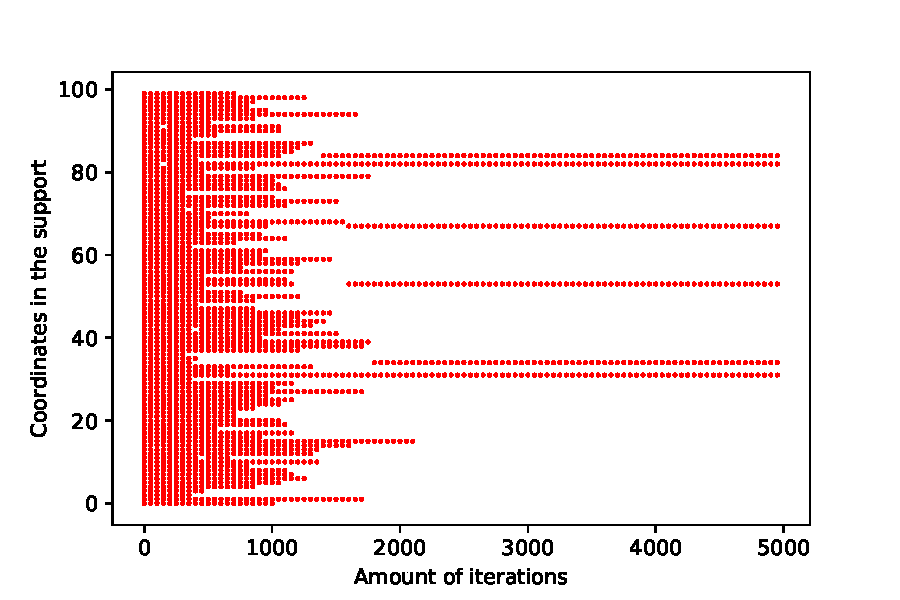
\includegraphics{basics_2/l1_supp.pdf}
\caption{$\ell_1$ identification}
\label{fig:l1supp}
\end{figure}

% \input{Article/l1_identification.tex}

In Figure~\ref{fig:l1supp} we can see how support changes during proximal gradient descent for LASSO problem 
$$
\min~\frac12\|Ax-b\|_2^2 + \lambda_1\|x\|_1
$$
for random generated matrix $A\in\mathbb{R}^{100\times100}$ and vector $b\in\mathbb{R}^{100}$ and hyperparameter $\lambda_1$ chosen to reach $6\%$ of density (amount of non-zero coordinates) of the final solution.
Starting from $500^{\text{th}}$ iteration the support of iterates begins to change and becomes stable after $2000$.


Another important example of sparsity inducing regularizer is $1$-d $\mathbf{TV}$ regularizer.
\begin{example}[$\mathbf{TV}$ regularizer]
It is known that if $r$ is $1$-d $\mathbf{TV}$ regularizer
\begin{equation}\label{eq:tvreg}
    r(x) = \sum\limits_{i=1}^{n-1}|x_{[i]} - x_{[i+1]}|
\end{equation}
it enforces variation sparsity.	

In this case the amount of jumps (blocks) in optimal solution $x^\star$ will be small, where
\begin{equation}
\jumps(x)\stackrel{\triangle}{=} \left\{i\in [2,n]\,| x_{[i]} \neq x_{[i-1]} \right\}.	
\end{equation}

Let us define collection $\M = \{\M_i\}_{1\leq i\leq d}$ as the set of all subspaces $\M_i$ with the fixed block structure i.e. $\jumps(x) = \jumps(y)$ for all $x,y\in \M_i$. In case of this collection, identification result \eqref{eq:identification_result} can be reformulated as
\begin{equation}\label{eq:ident_tv}
    \jumps(x^\star) \subseteq \jumps(x^k) \subseteq \bigcup_{u\in\mathcal{B}(u^\star,\varepsilon)} \jumps(\prox_{\gamma r}(u)).
\end{equation}

To prove this it is enough to show that
\begin{equation}\label{eq:s_to_jumps}
    \S(x)\leq\S(y) \iff \jumps(x)\subseteq\jumps(y),
\end{equation}
which proves exactly the same way as \eqref{eq:s_to_supp}.

\end{example}


% This result yields immediately that the iterates of the subspace descent method presented in Section~\ref{sec:algo} will reach some ``structure'': they will belong to some of the subspaces in $\M$ after some finite time with probability one, and these subspaces are sandwiched between the two extremes families of subspaces controlled by the pair $(x^\star, u^\star)$. 
The Theorem \ref{th:identification} explains that iterates of any converging proximal algorithm will eventually be sandwiched between two extremes families of subspaces controlled by the pair $(x^\star, u^\star)$.



%\section{Useful tools for stochastic processes analysis.}\label{sec:basics-stoch-basics}
{\color{blue}
In this section, we recall some definitions and results from the probability theory that we will use in our further proofs.

Let us start from the law of total expectation \cite[Chapter V, Section $4$]{kolmogorov1933grundbegriffe}.

\begin{lemma}[Tower property]\label{lm:tower_exp}
For any random variables $X$ and $Y$, we have $\EE[X] = \EE\left[\EE[X|Y]\right]$.
\end{lemma}
\begin{proof}[Proof of Lemma \ref{lm:tower_exp}]
    Let us provide the proof for discrete random variables only.
\begin{align}
\EE[X] &= \sum_x x P(X=x) = \sum_x x\sum_yP(X=x)\&P(Y=y) = \sum_x\sum_y x P(X=x)\&P(Y=y)\nonumber\\
&= \sum_x\sum_y P(Y=y)x\frac{P(X=x\&Y=y)}{P(Y = y)}  = \sum_y P(Y=y) \sum_x xP(X=x\&Y=y)\nonumber\\
& = \sum_y P(Y=y) \EE[X|Y=y] = \EE\left[\EE[X|Y]\right],
\end{align}
which finishes the proof.
\end{proof}

Now, let us present the notion of almost surely convergence \cite{stout1974almost}.
\begin{definition}[Almost sure convergence]
    We say that the sequence $\left\{X_t\right\}$ of random variables $X_t:\Omega\rightarrow \mathcal{S}$ converges almost surely (a.s.) to $X\in\mathcal{S}$ if 
    $$
    \mathbf{P}\left[\omega\in\Omega:\lim_{n\rightarrow\infty}X_n(s) = X\right] = 1.
    $$
\end{definition}

The following theorem allows proving almost sure convergence for almost supermartingales \cite[Theorem $1$]{robbins1971convergence}.
\begin{theorem}\label{th:r-s_theorem}
Consider probability space $(\Omega, \mathcal{F}, \PP)$ with the sequence of $\sigma$-algebras $\FF_1\subset\FF_2\subset\ldots$. For each $n = 1,2,\ldots$ let $z_n, \beta_n, \xi_n,$ and $\zeta_n$ be non-negative $\FF_n$-measurable random variables such that
\begin{equation}\label{eq:a-super-martingale}
\EE[z_{n+1}|\FF_n]\leq z_n(1+\beta_n) + \xi_n - \zeta_n.
\end{equation}
Assume that $\sum_{i=1}^\infty \beta_i<\infty$ and $\sum_{i=1}^\infty \xi_i<\infty$ then $\lim_{n\rightarrow\infty}z_n$ exist and is finite and $\sum_{i=1}^\infty \zeta_i<\infty$ a.s.
\end{theorem}
}

